\documentclass{beamer}
\mode<presentation>
%% \mode<handout>{\setbeamercolor{background canvas}{bg=black!5}}
\usetheme{CambridgeUS}
\usecolortheme{dolphin}

\usepackage{bstyle}
\graphicspath{{figs/}}

\title[Horse Induction]{Hay is for Horses}
\subtitle{And, All Horses are the Same Color}
\author[B.\ T.\ Fasy]{Prof.\ Brittany Terese Fasy}
\institute[MSU]{School of Computing \& Dept.\ of Mathematical Sciences}
\date{}

\begin{document}

\frame<1>{
    \frametitle{Prof.~Brittany Terese Fasy}
\begin{block}{}

    \begin{table}[]
        \begin{tabular}{ll}
            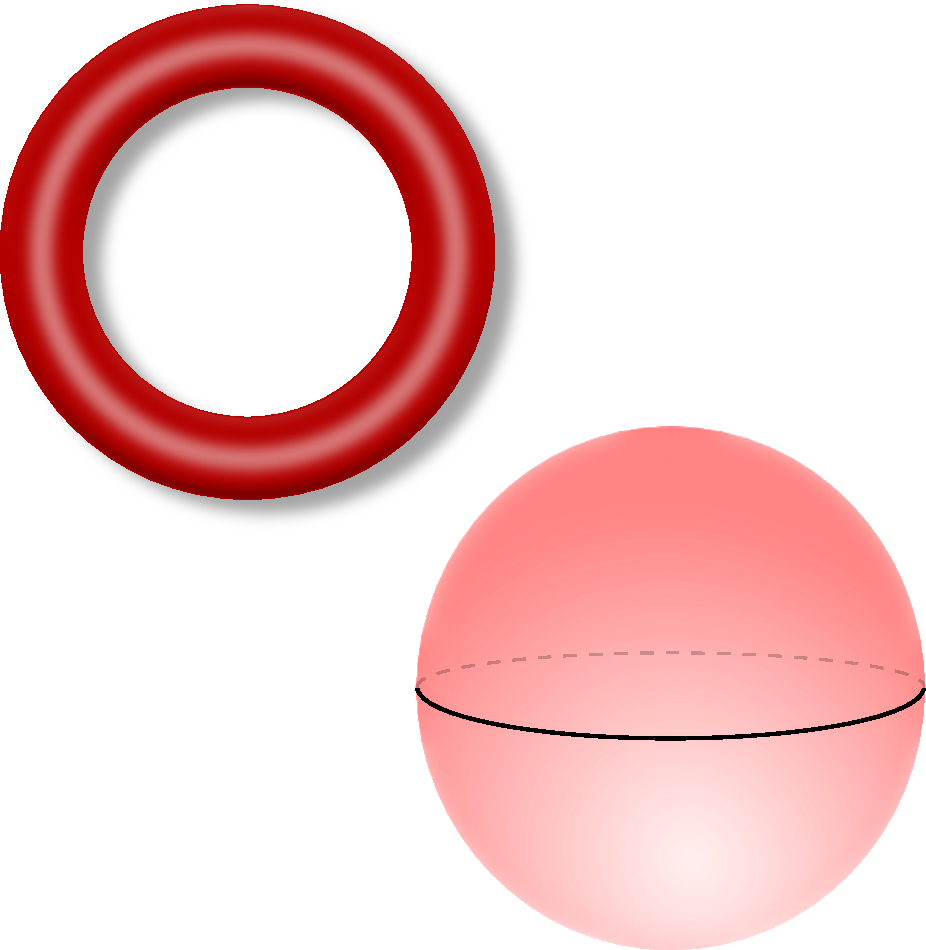
\includegraphics[height=.35in,width=.5in]{hom-2d}
            &
            \shortstack[l]{B.S., Mathematics and Computer Science \\
            Saint Joseph's University, Philadelphia, PA}\\
            & \\
            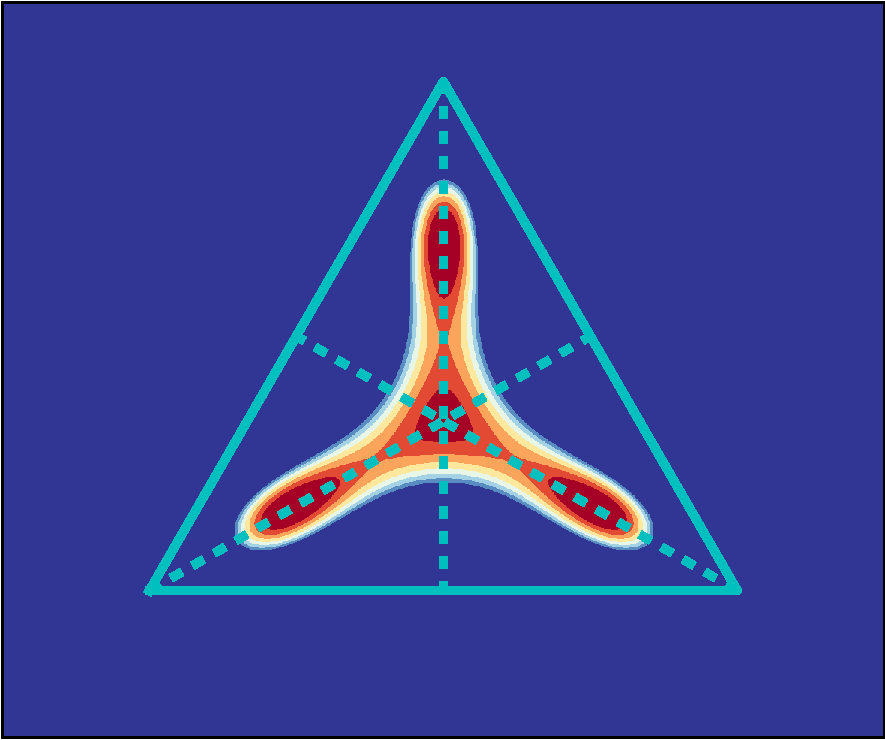
\includegraphics[height=.35in,width=.5in]{kern-gauss}
            &
            \shortstack[l]{Ph.D., Computer Science, Duke University \\
            Adviser: Herbert Edelsbrunner  (IST Austria)} \\
            & \\

            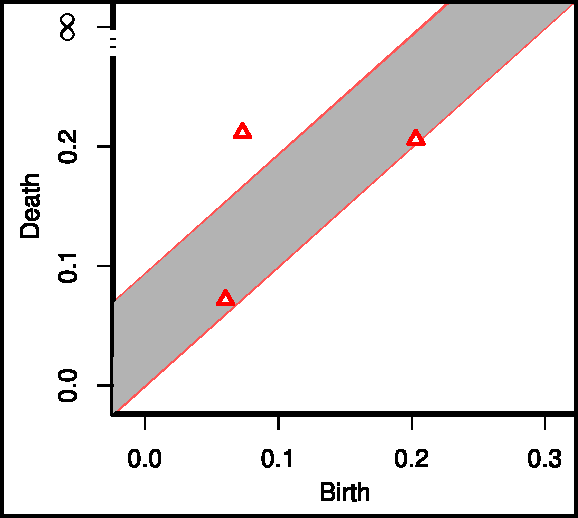
\includegraphics[height=.35in,width=.5in]{balls-dgm-threshold}
            &
            \shortstack[l]{
            Postdoc: Carnegie Mellon University\\
            CMU TopStat (stat.cmu.edu/topstat)}\\
            & \\

            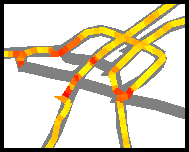
\includegraphics[height=.35in,width=.5in]{athens-zoom}
            &
            \shortstack[l]{Postdoc: Tulane University\\
            Applications of TDA}\\
            & \\

            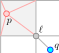
\includegraphics[height=.35in,width=.5in]{boundcollision}
            &
            \shortstack[l]{
            Associate Professor: Montana State University\\
            Searching, Directed Topology, Homotopy Area, ...}
        \end{tabular}
    \end{table}
\end{block}
}

\frame{
    \frametitle{Who are you?}
    \begin{block}{}
        \begin{enumerate}
            \item State your name, major, and expected graduation.
            \item Why are you taking this class?
            \item Exchange contact info!
        \end{enumerate}
    \end{block}
}

\frame{
    \frametitle{Meet another classmate}
    \begin{block}{}
        \begin{enumerate}
            \item State your name, major, and expected graduation.
            \item What is an algorithm?
            \item Exchange contact info!
        \end{enumerate}
    \end{block}
}

\frame{
    \frametitle{}
    \begin{block}{}
        Induction Recap
    \end{block}
}



\begin{frame}
\titlepage
\end{frame}

\begin{frame}
\frametitle{Kyoto, Summer 2014}
\begin{columns}
 \column{.45\textwidth}
 \centering
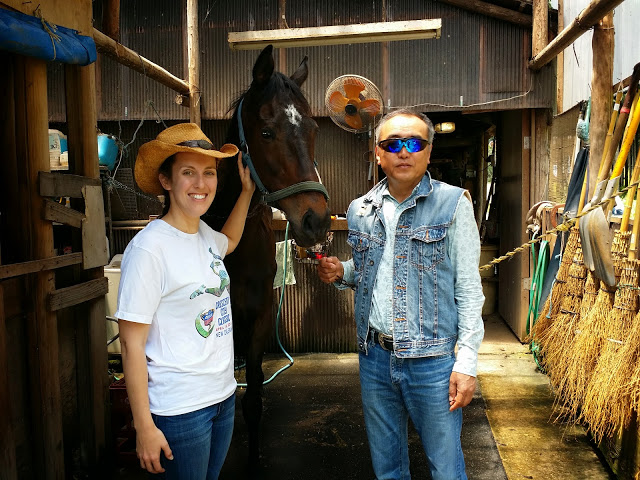
\includegraphics[width=\textwidth]{japan}
  \column{.45\textwidth}
  \centering
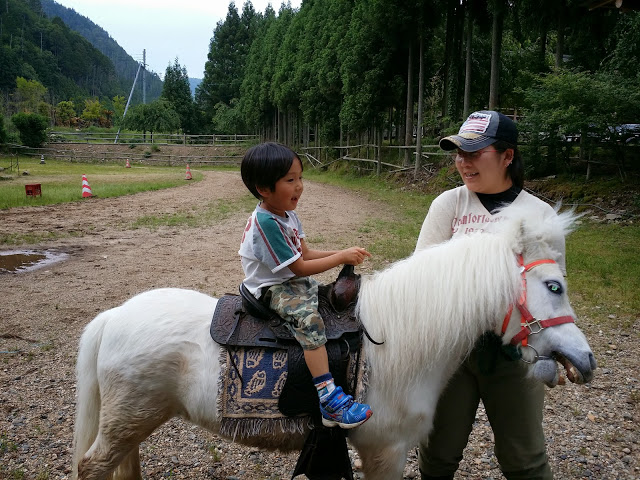
\includegraphics[width=\textwidth]{pony}
\end{columns}

\pause
\begin{block}{But Wait!}
 All horses (and ponies) are the same color!
\end{block}
\end{frame}

\frame{
\frametitle{Reminder: Proof by Induction}


\begin{block}{5 Steps}
\begin{columns}
 \column{.4\textwidth}
 {\bf
 1.~Claim:\\
 2.~Base Case:\\
 3.~Inductive Assumption:\\
 4.~Inductive Step:\\
 5.~Conclude! \pause
 }
 \column{.6\textwidth}
 Property A holds for all $n \geq n_0$.\\ \pause
 Show Property A holds for $n_0$.\\ \pause
 Assume Property A holds for some $n=k$.\\ \pause
 Prove that Property A holds for $n=k+1$.\\
    ~~
\end{columns}
\end{block}

}

\frame{
    \frametitle{Proofs by Induction}

    \begin{block}{Problem I}
        For all integers $n \geq 0$, $\sum_{i=0}^n i = \frac{n(n+1)}{2}$.
    \end{block}

    \begin{block}{Problem II}
        For all integers $n \geq 2$, $n^2 \geq n+1$.
    \end{block}

    \begin{block}{Problem III}
        A tree with $n$ nodes has $n-1$ edges.
    \end{block}
}

\frame[label=horseinduction]{
\frametitle{Example of Proof by Induction}

\begin{block}{{\bf Claim:} ~~~~~~~~~~~~~~~~~~~~~~~~~ All horses are
the same color.}
\begin{columns}
 \column{.35\textwidth}
 {\bf
 Base Case:\\
 Inductive Assumption:\\
 Inductive Step:\\
 }
 \column{.6\textwidth}
 \onslide<1->{One horse is clearly one color.\\}%
 \onslide<2->{Any group of $k$ horses are the same color.\\}%
 \onslide<3->{Prove statement holds for $k+1$ horses.}%
\end{columns}
\end{block}

\begin{columns}
 \column{.45\textwidth}
 \onslide<1->{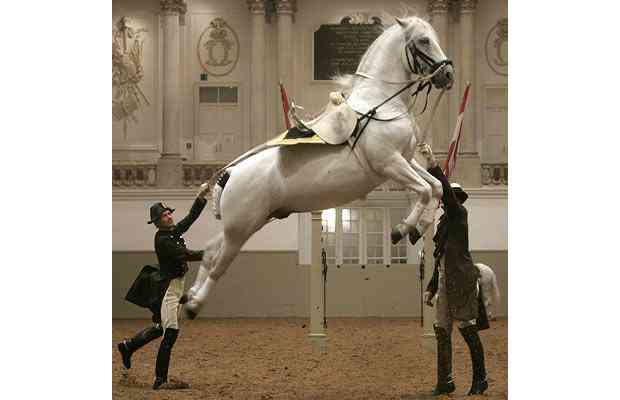
\includegraphics[width=\textwidth]{horse-jump}
 \\
 \footnotesize{http://www.telegraph.co.uk/}
 }%
 \column{.45\textwidth}
 \onslide<2->{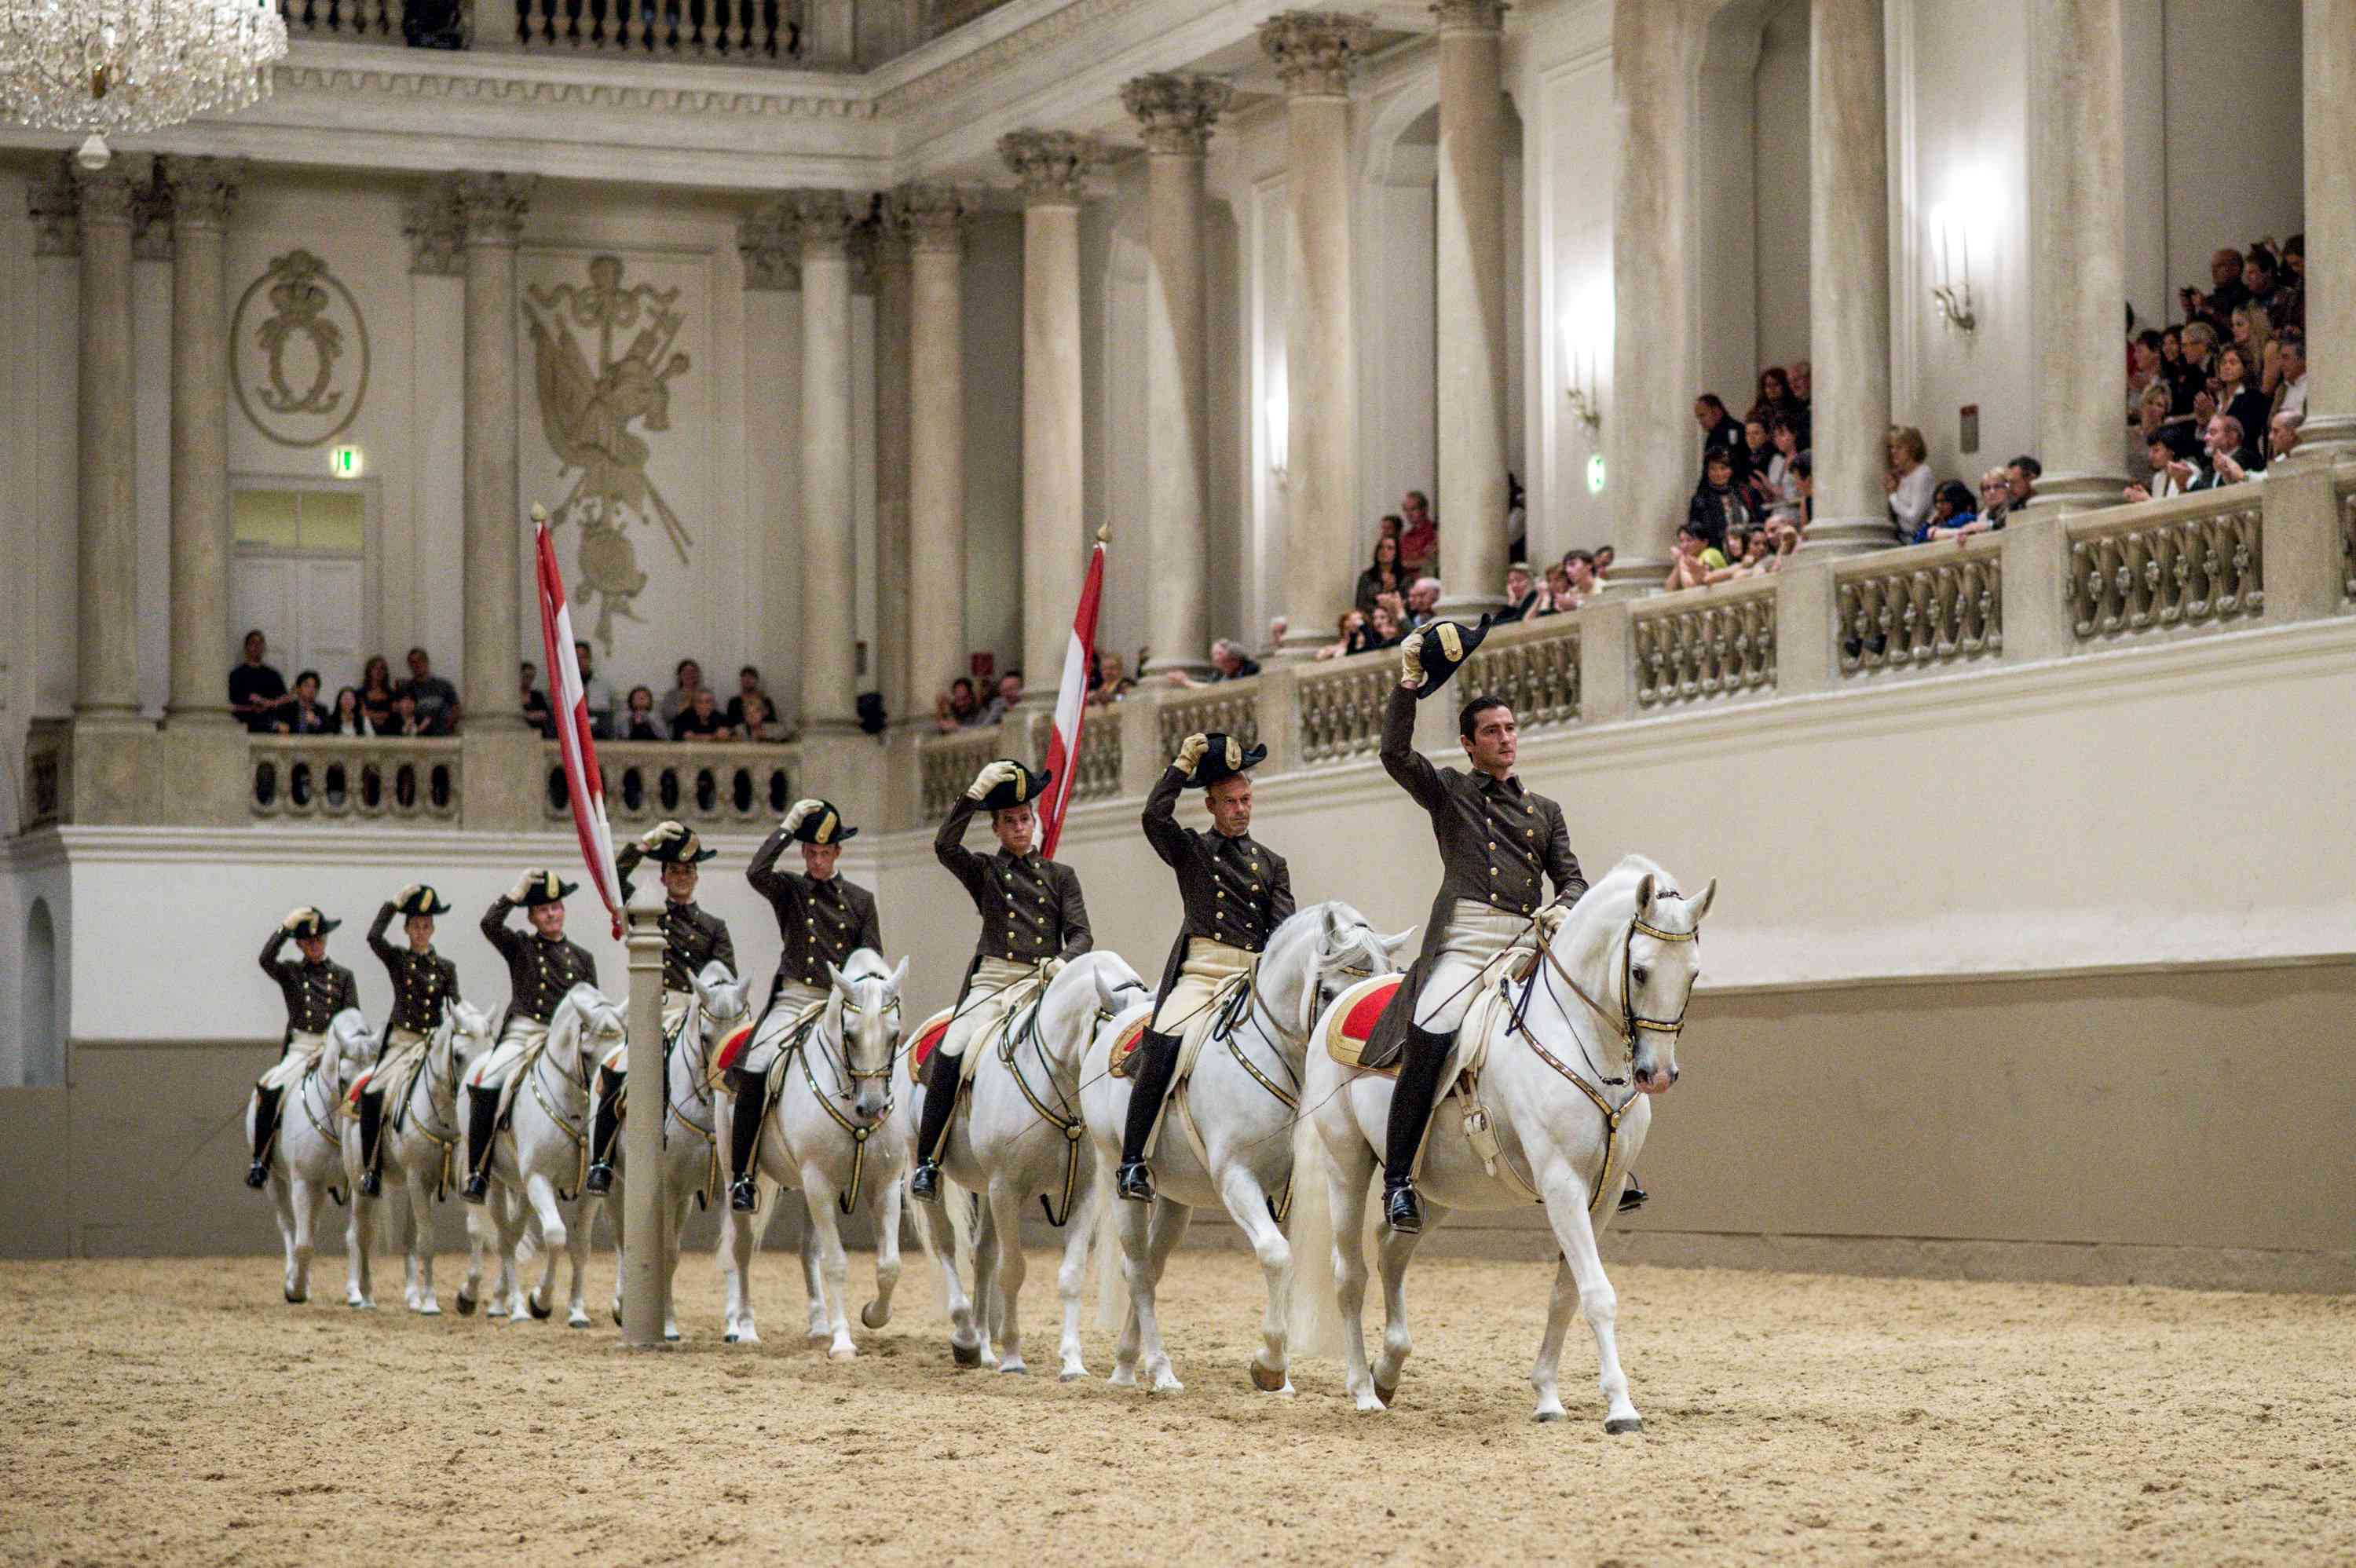
\includegraphics[width=\textwidth]{nhorses}
 \\
 \footnotesize{http://www.equestrianlifemagazine.co.uk/}
 }%
\end{columns}
}

\frame{
\frametitle{The Inductive Step}

\begin{block}{}
 \centering
 \only<1,4>{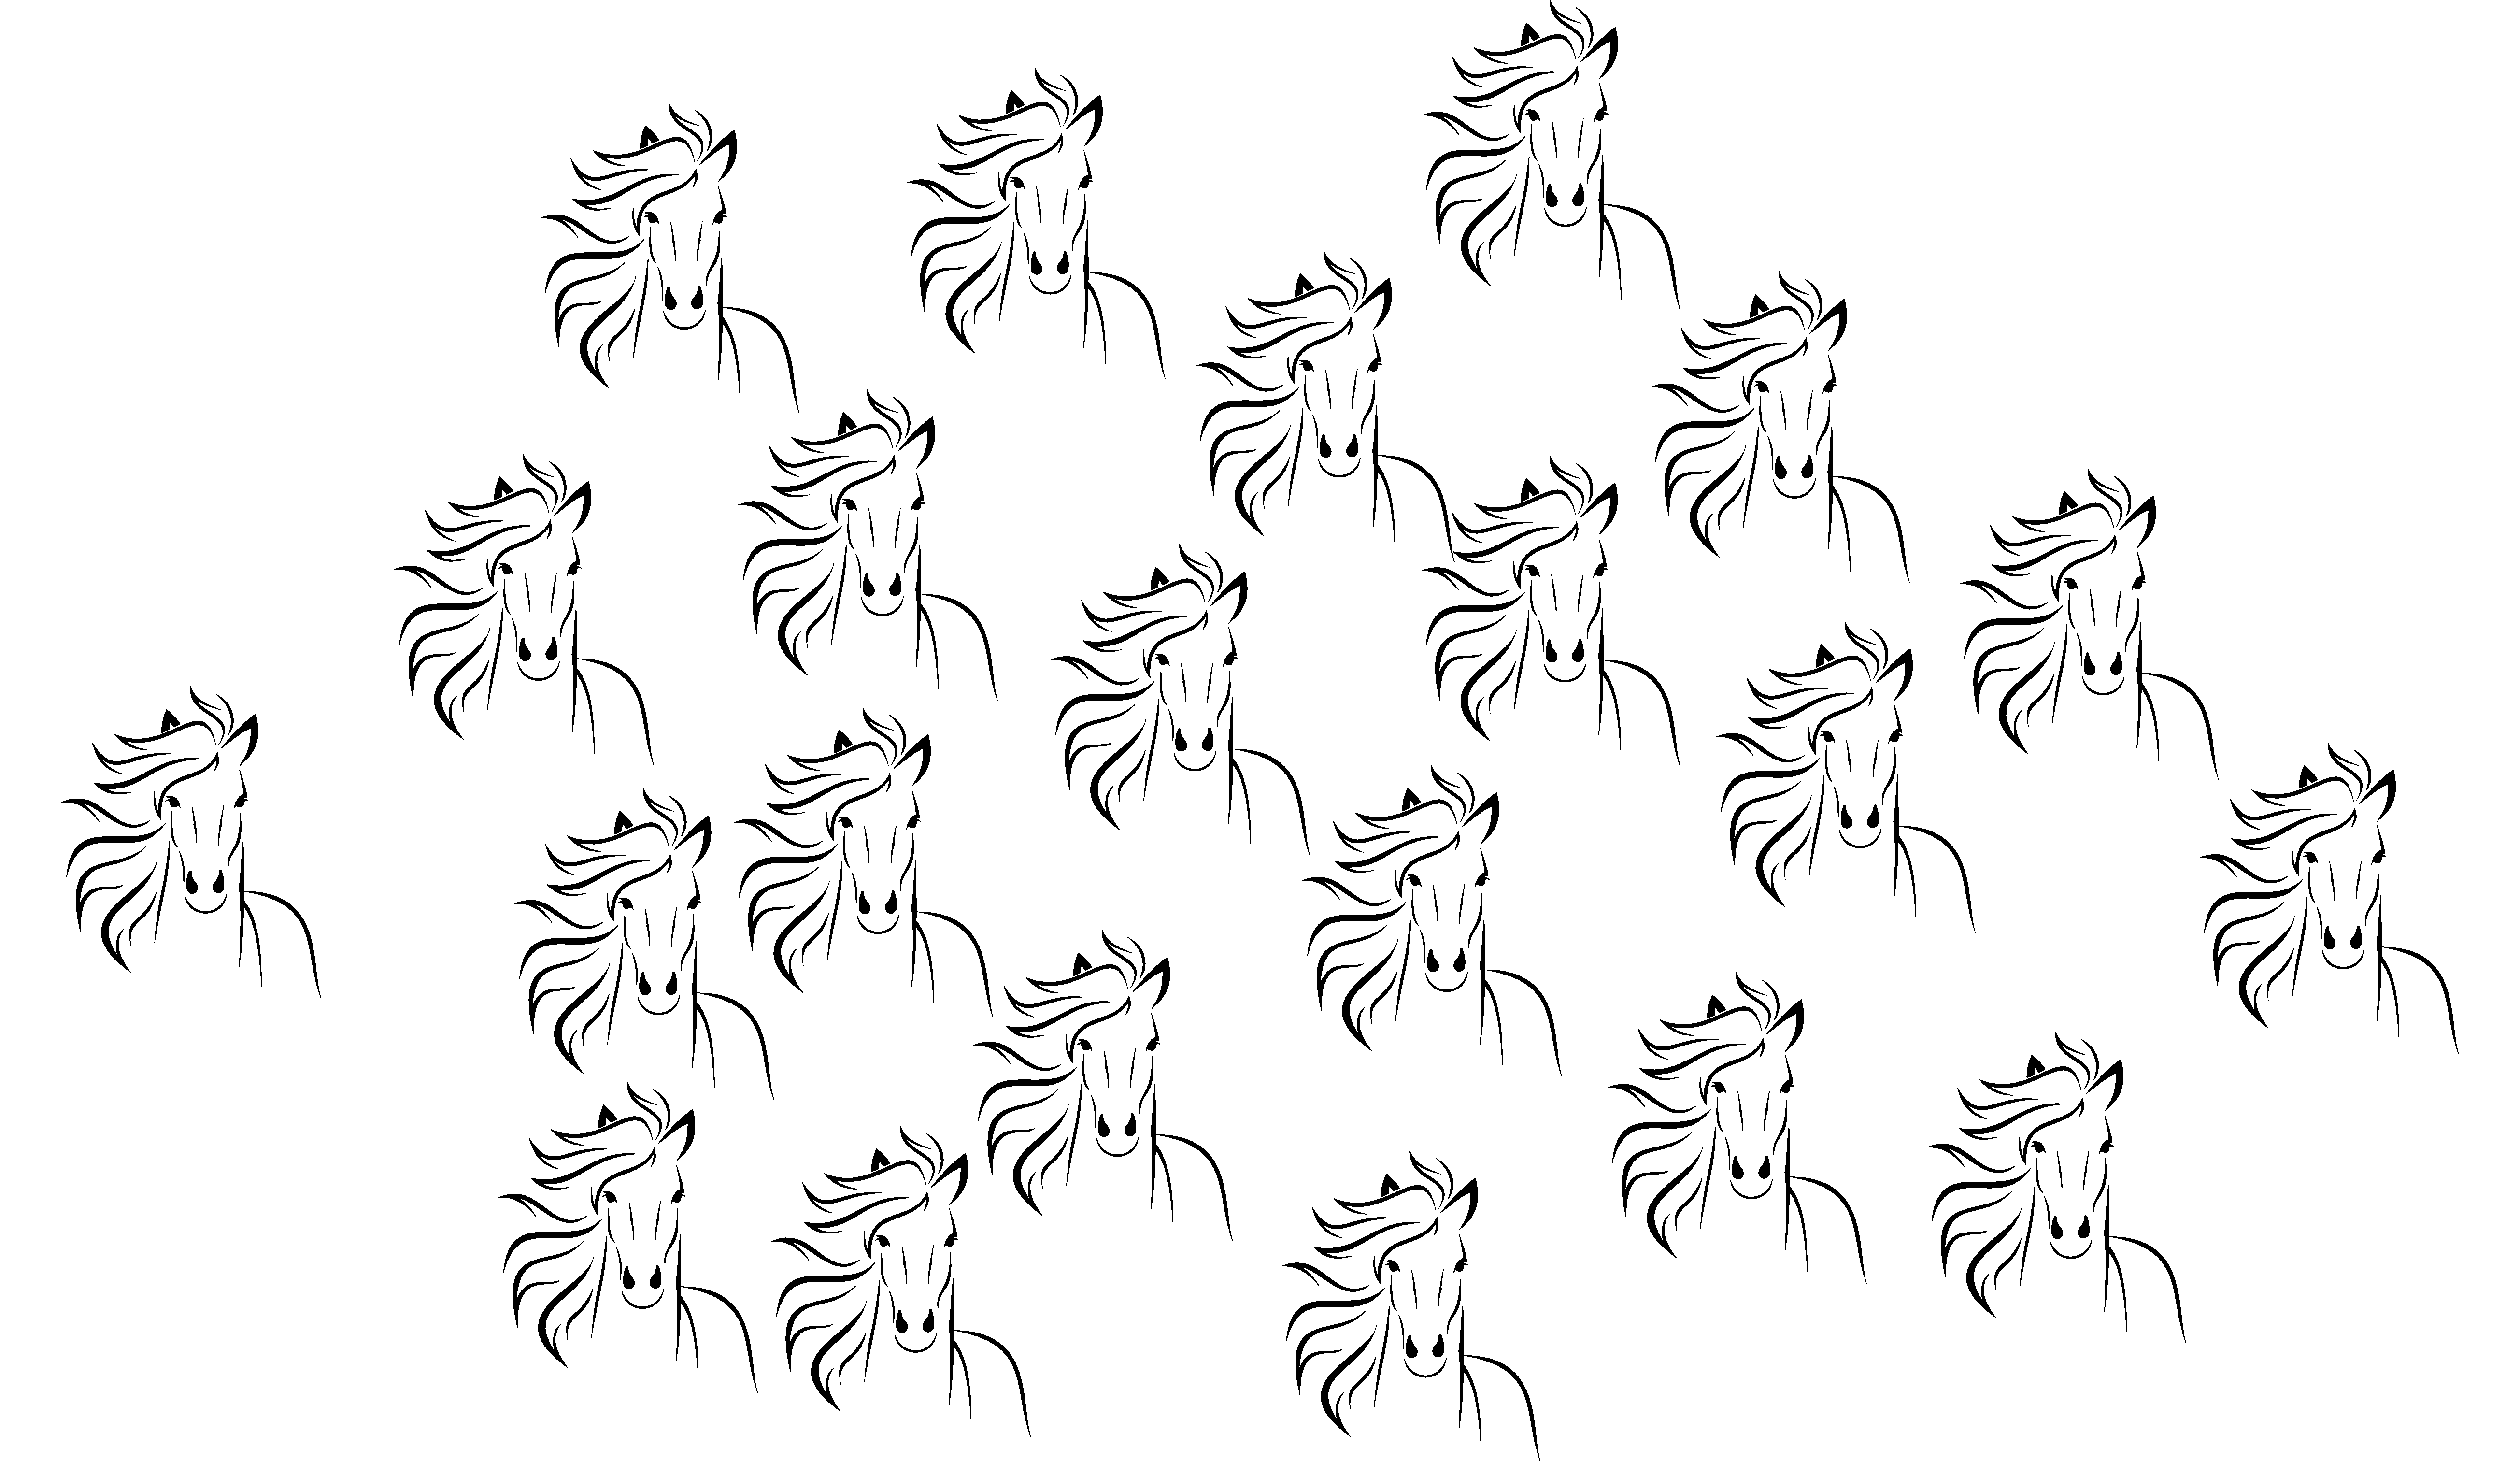
\includegraphics[height=2.5in]{pferd-weiss}}%
 \only<2>{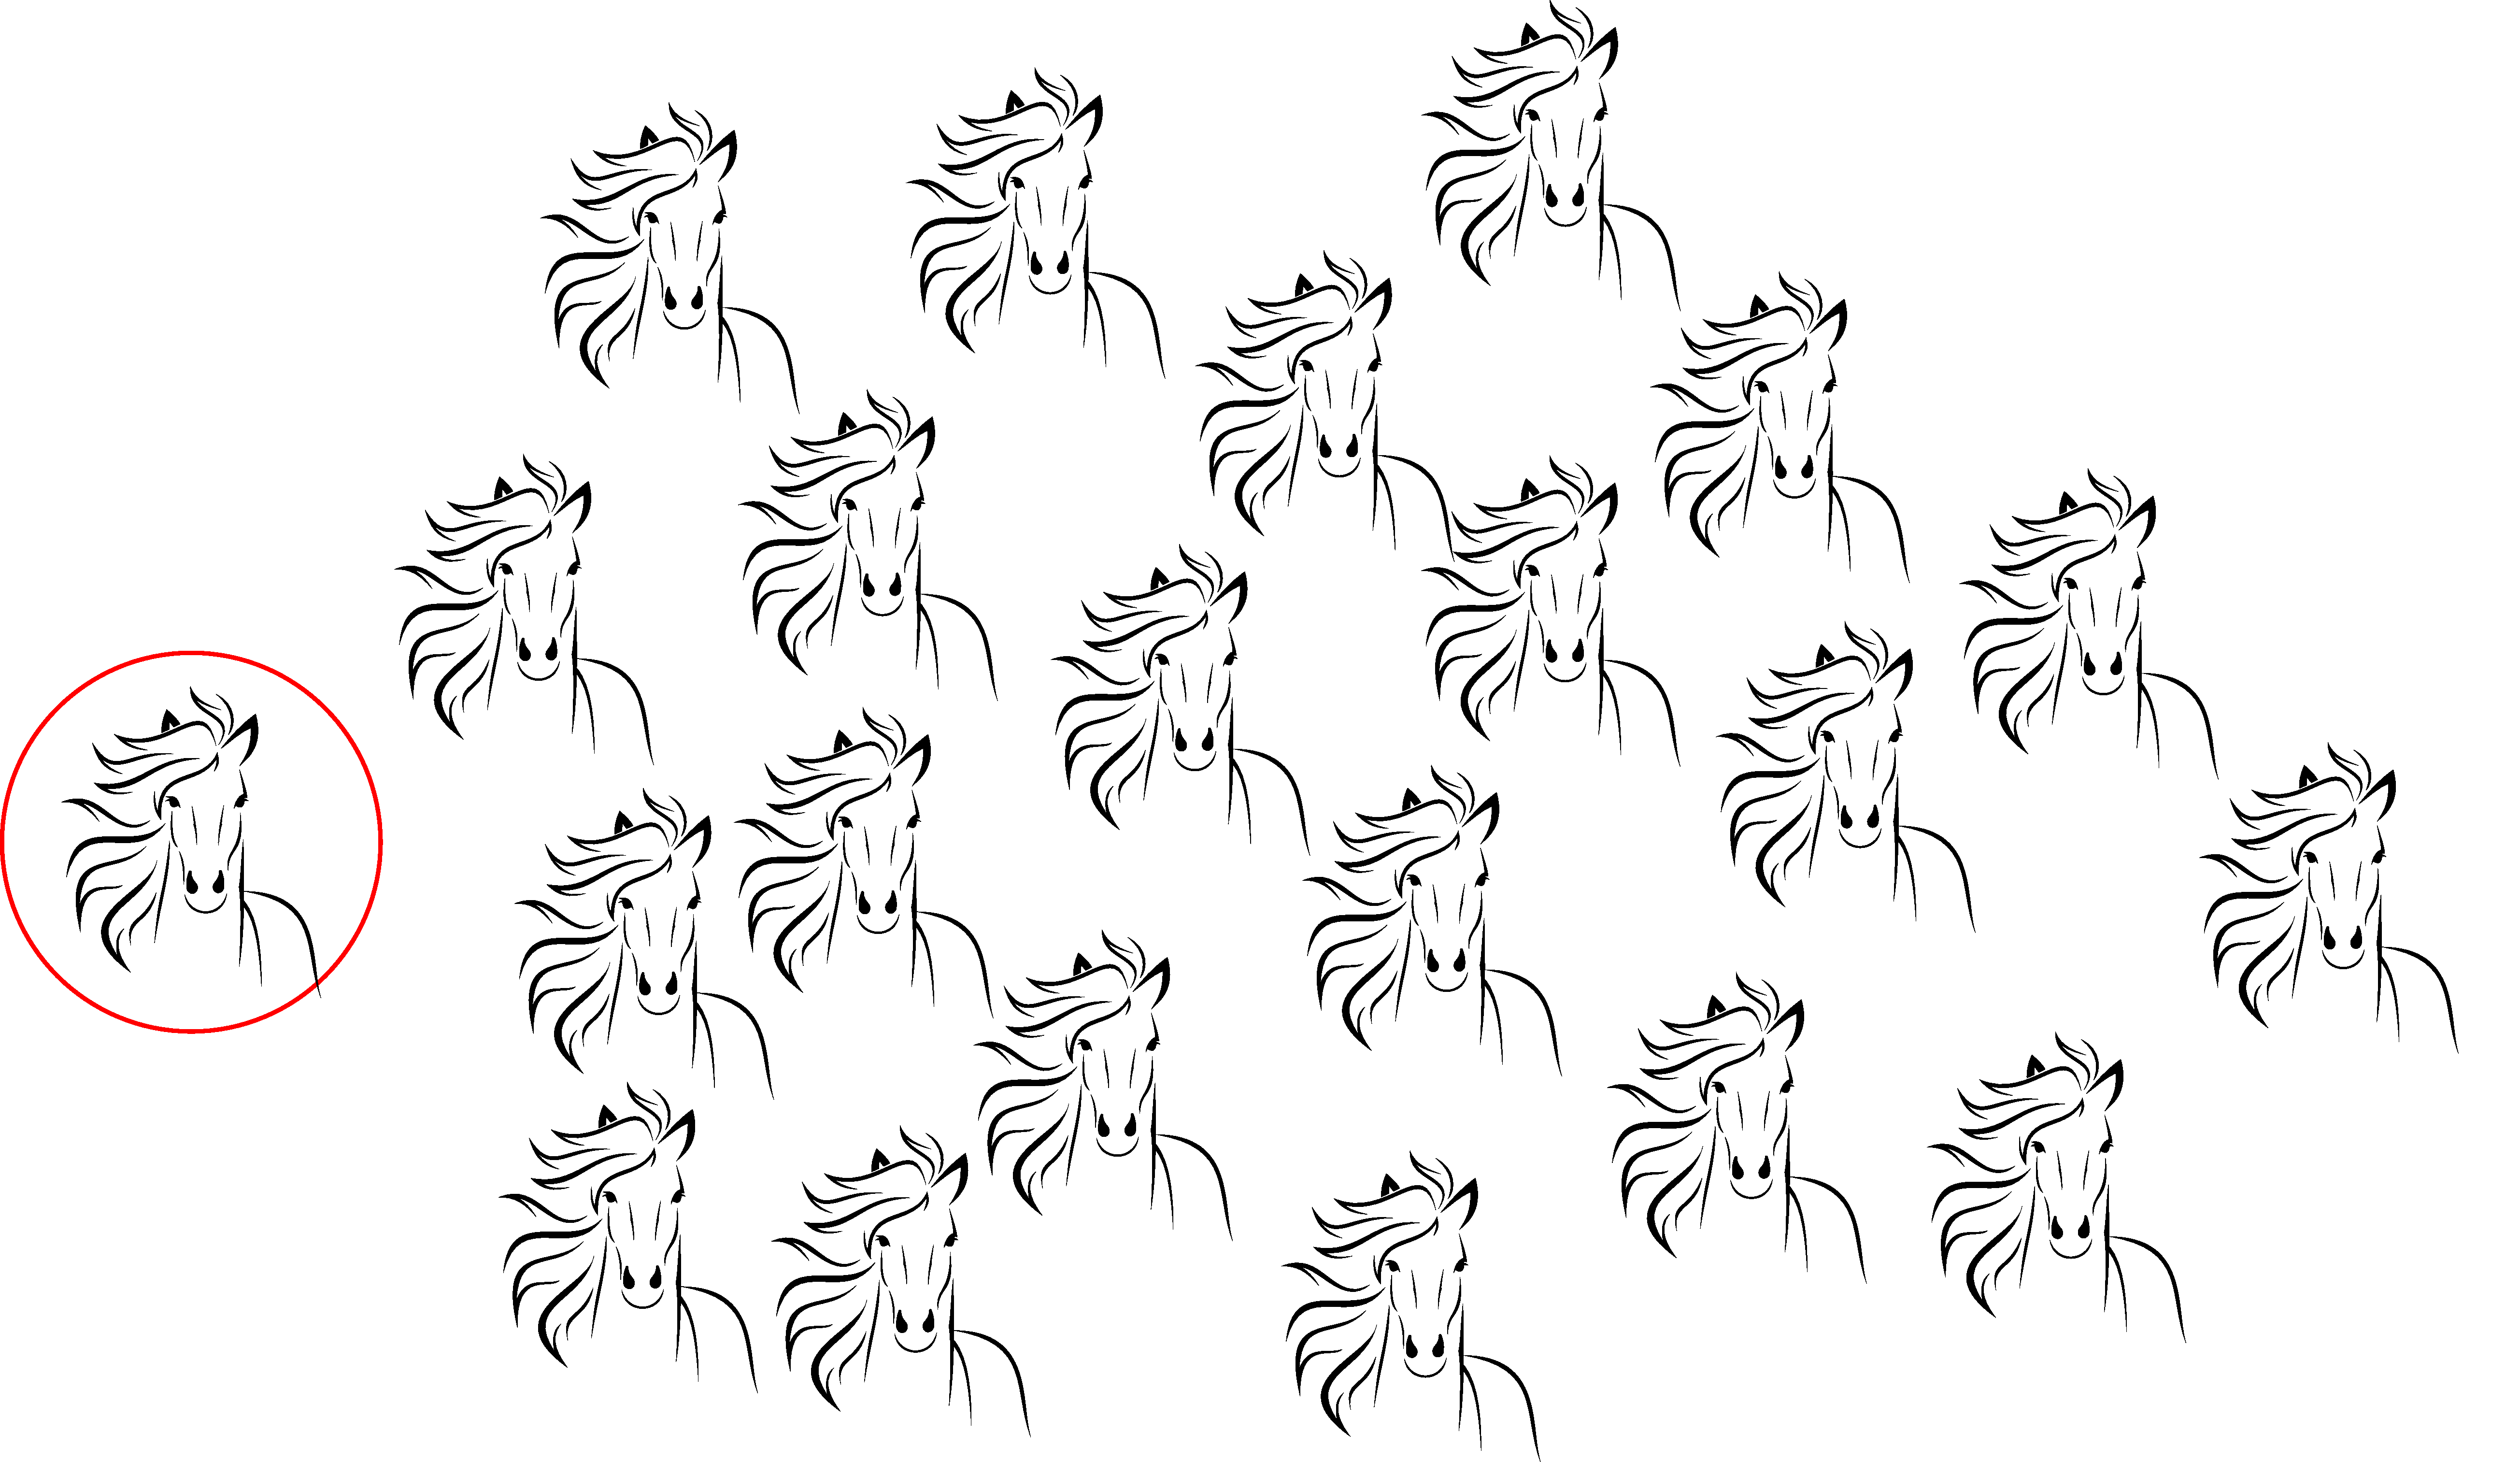
\includegraphics[height=2.5in]{pferd-weiss-selL}}%
 \only<3>{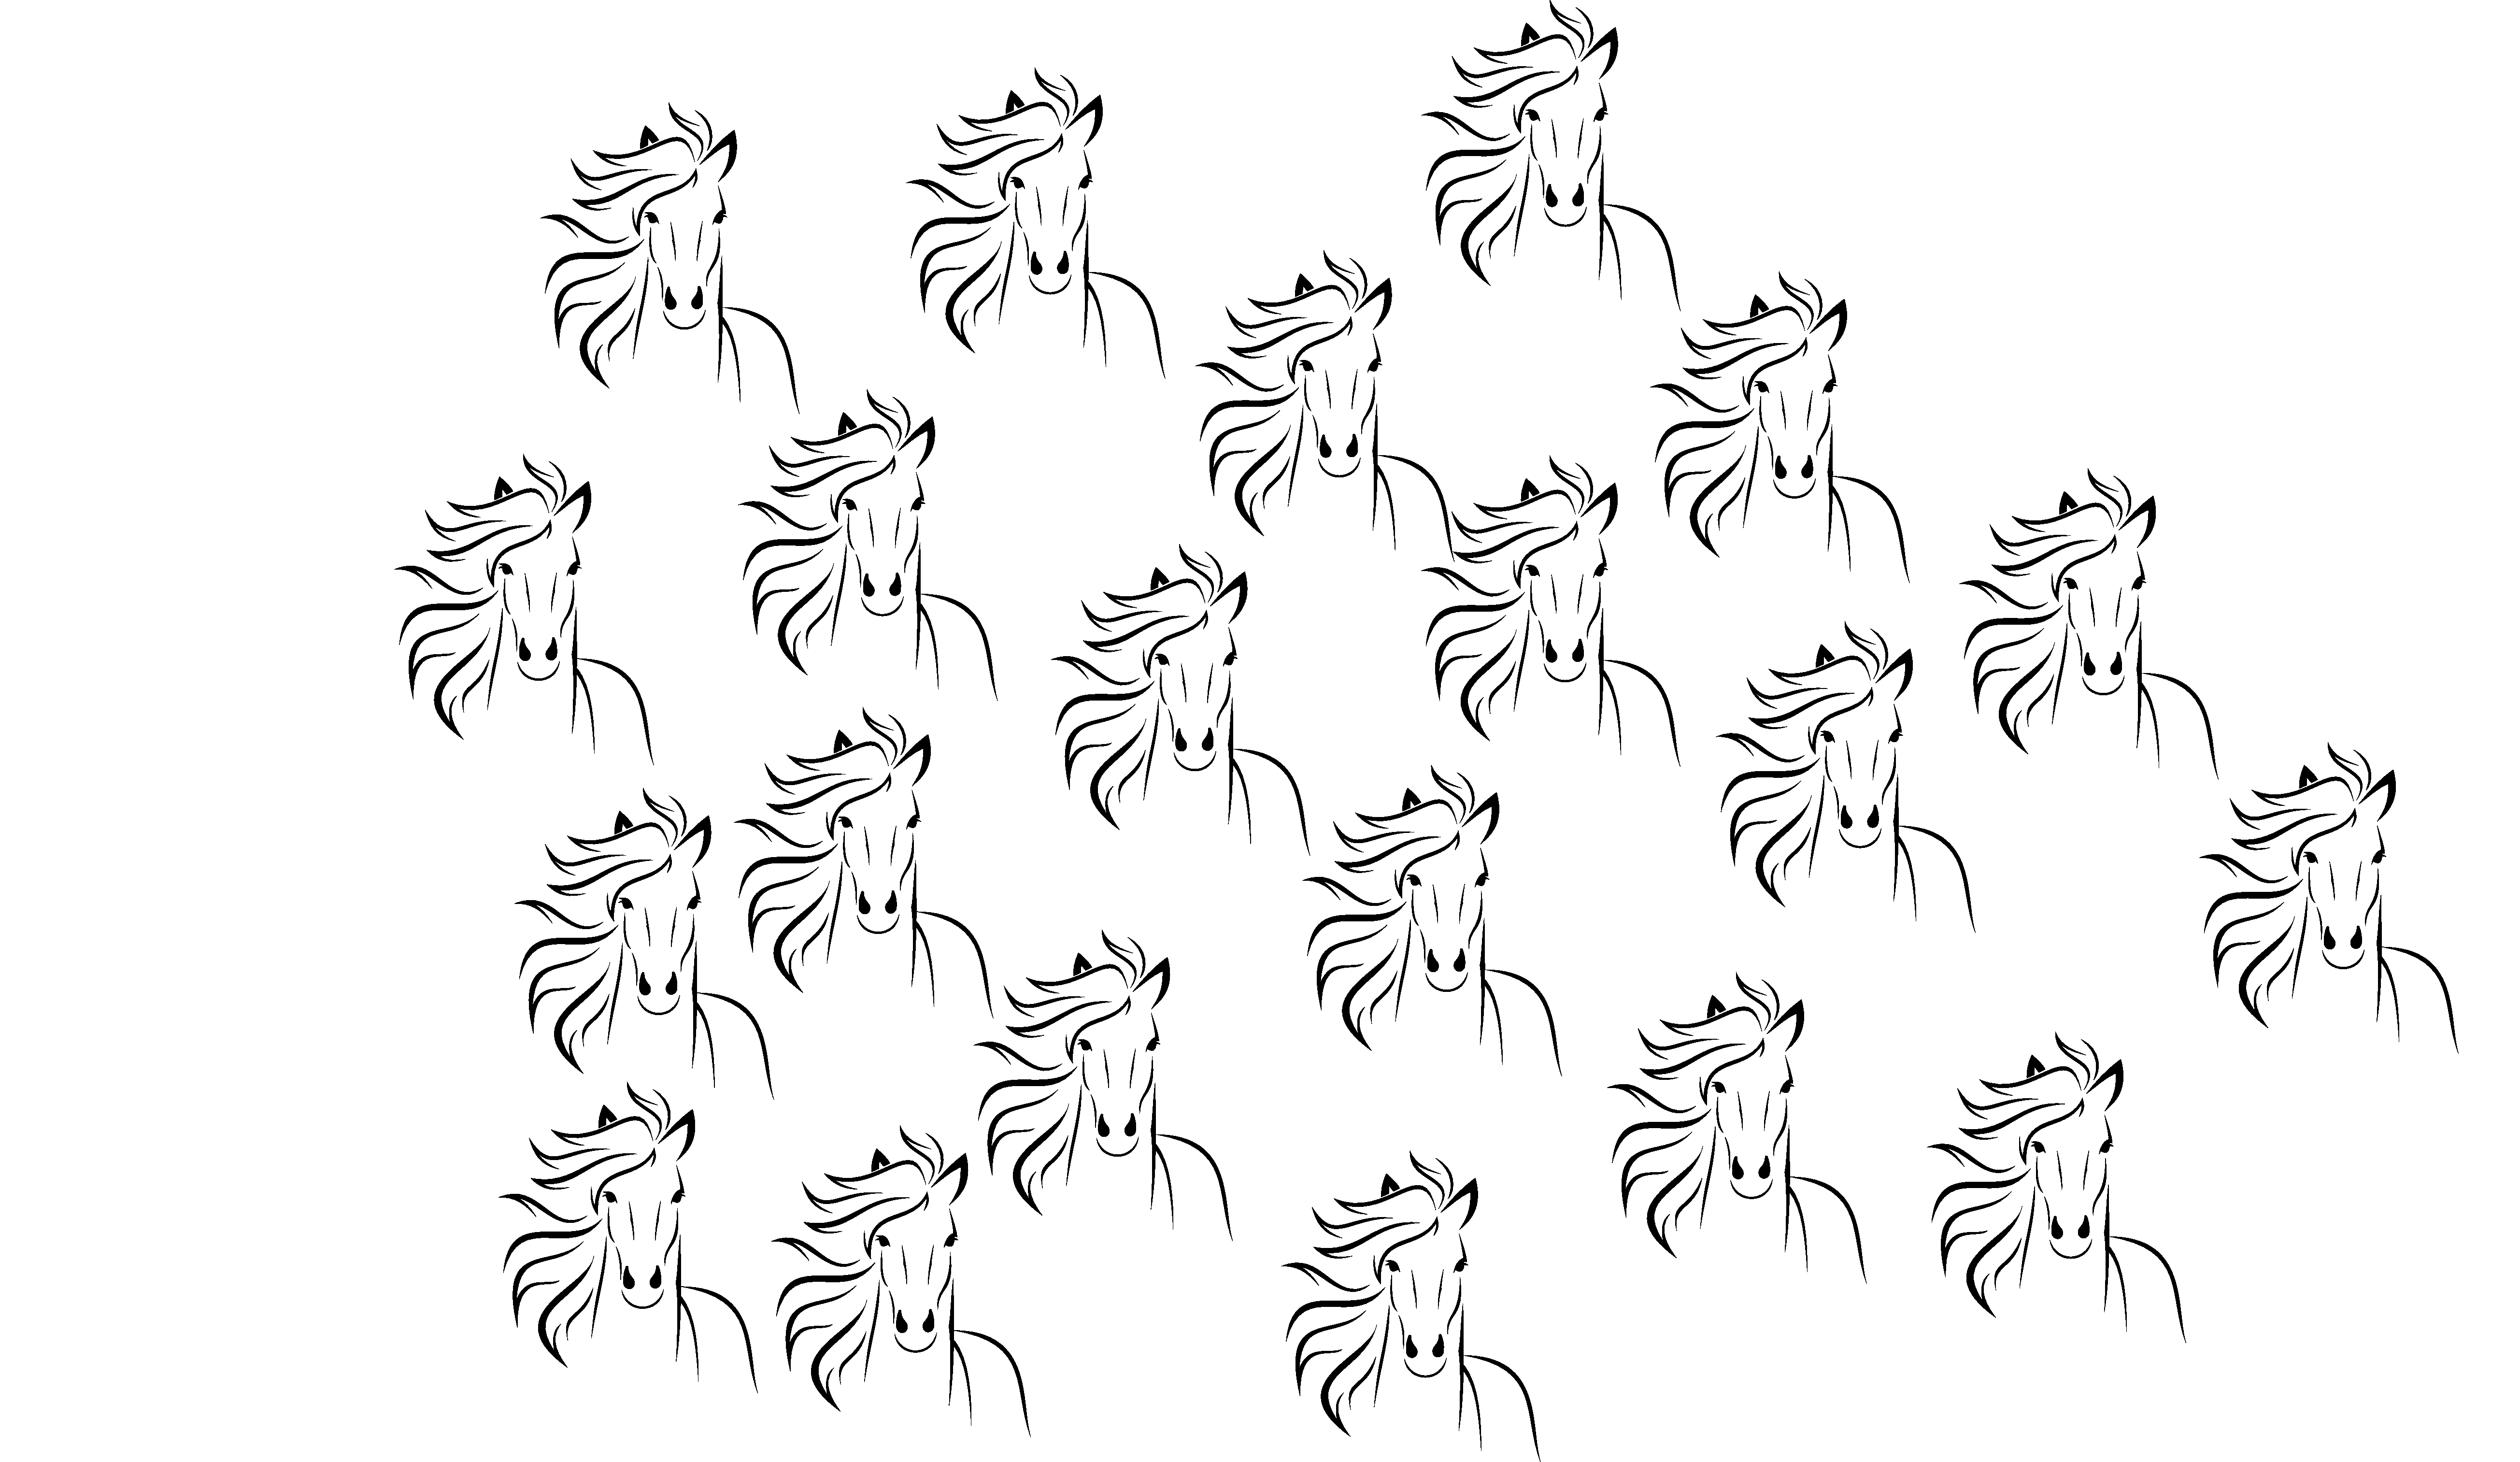
\includegraphics[height=2.5in]{pferd-weiss-remL}}%
 \only<5>{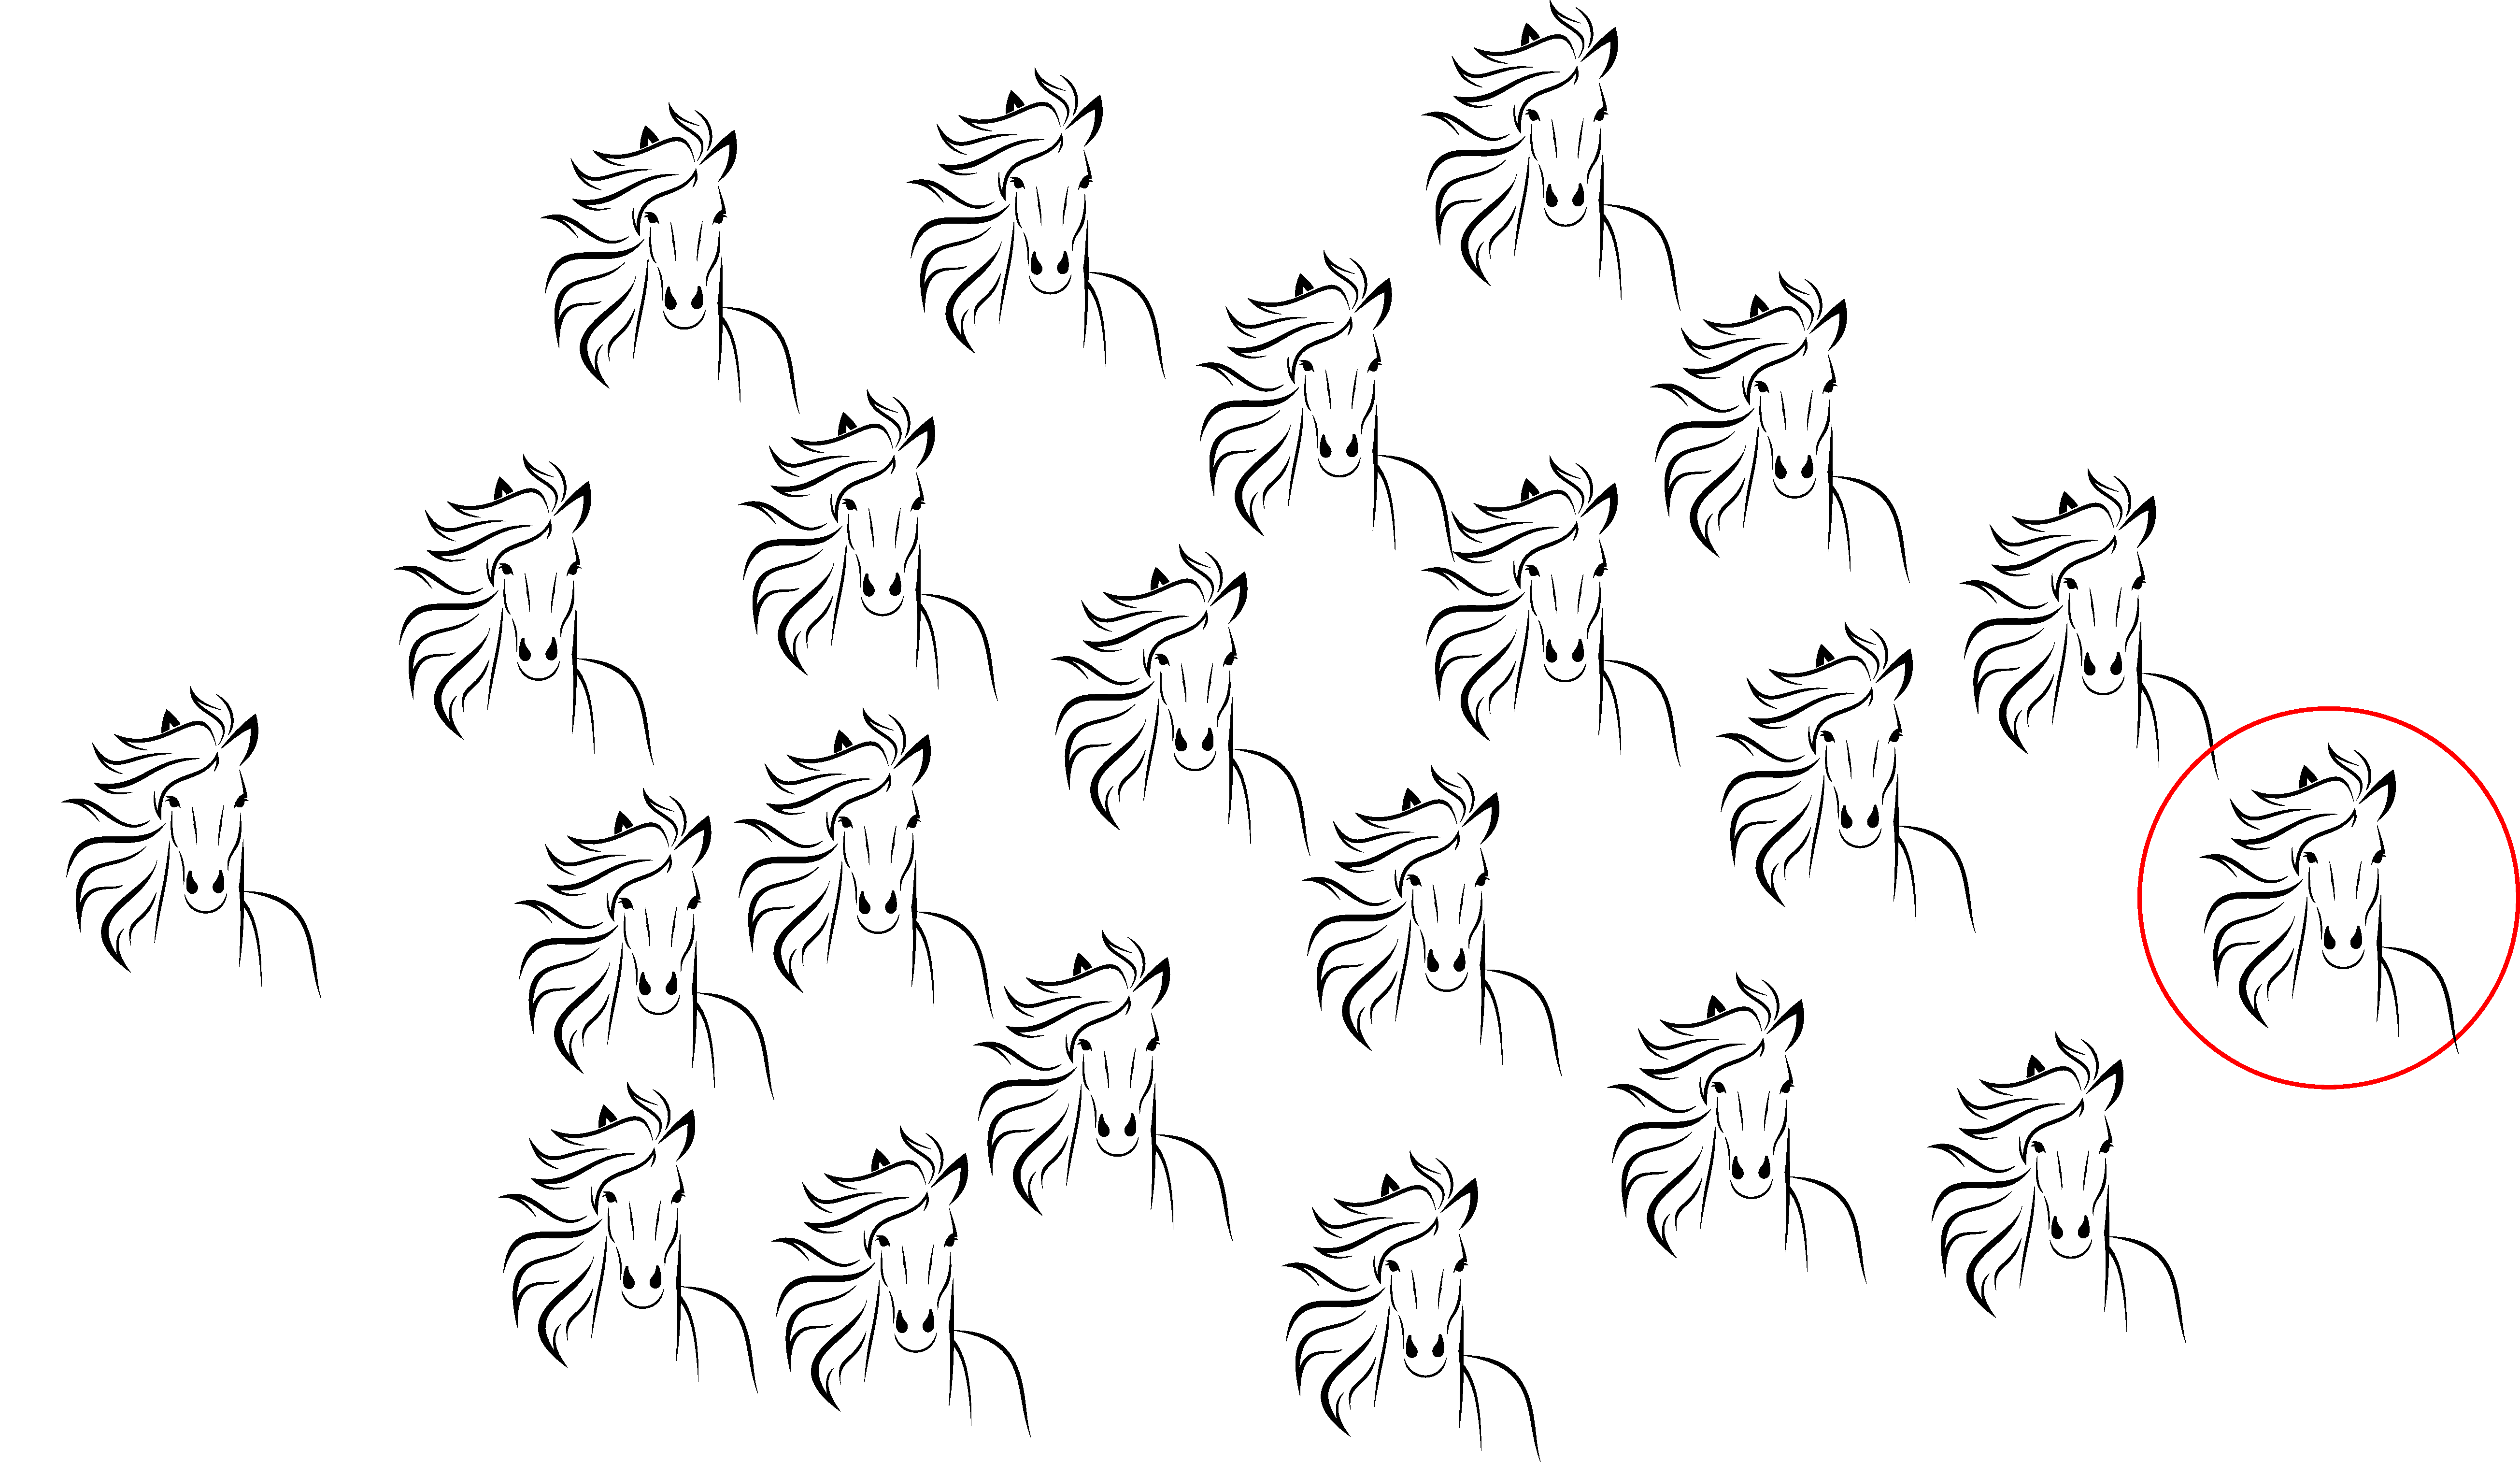
\includegraphics[height=2.5in]{pferd-weiss-selR}}%
 \only<6>{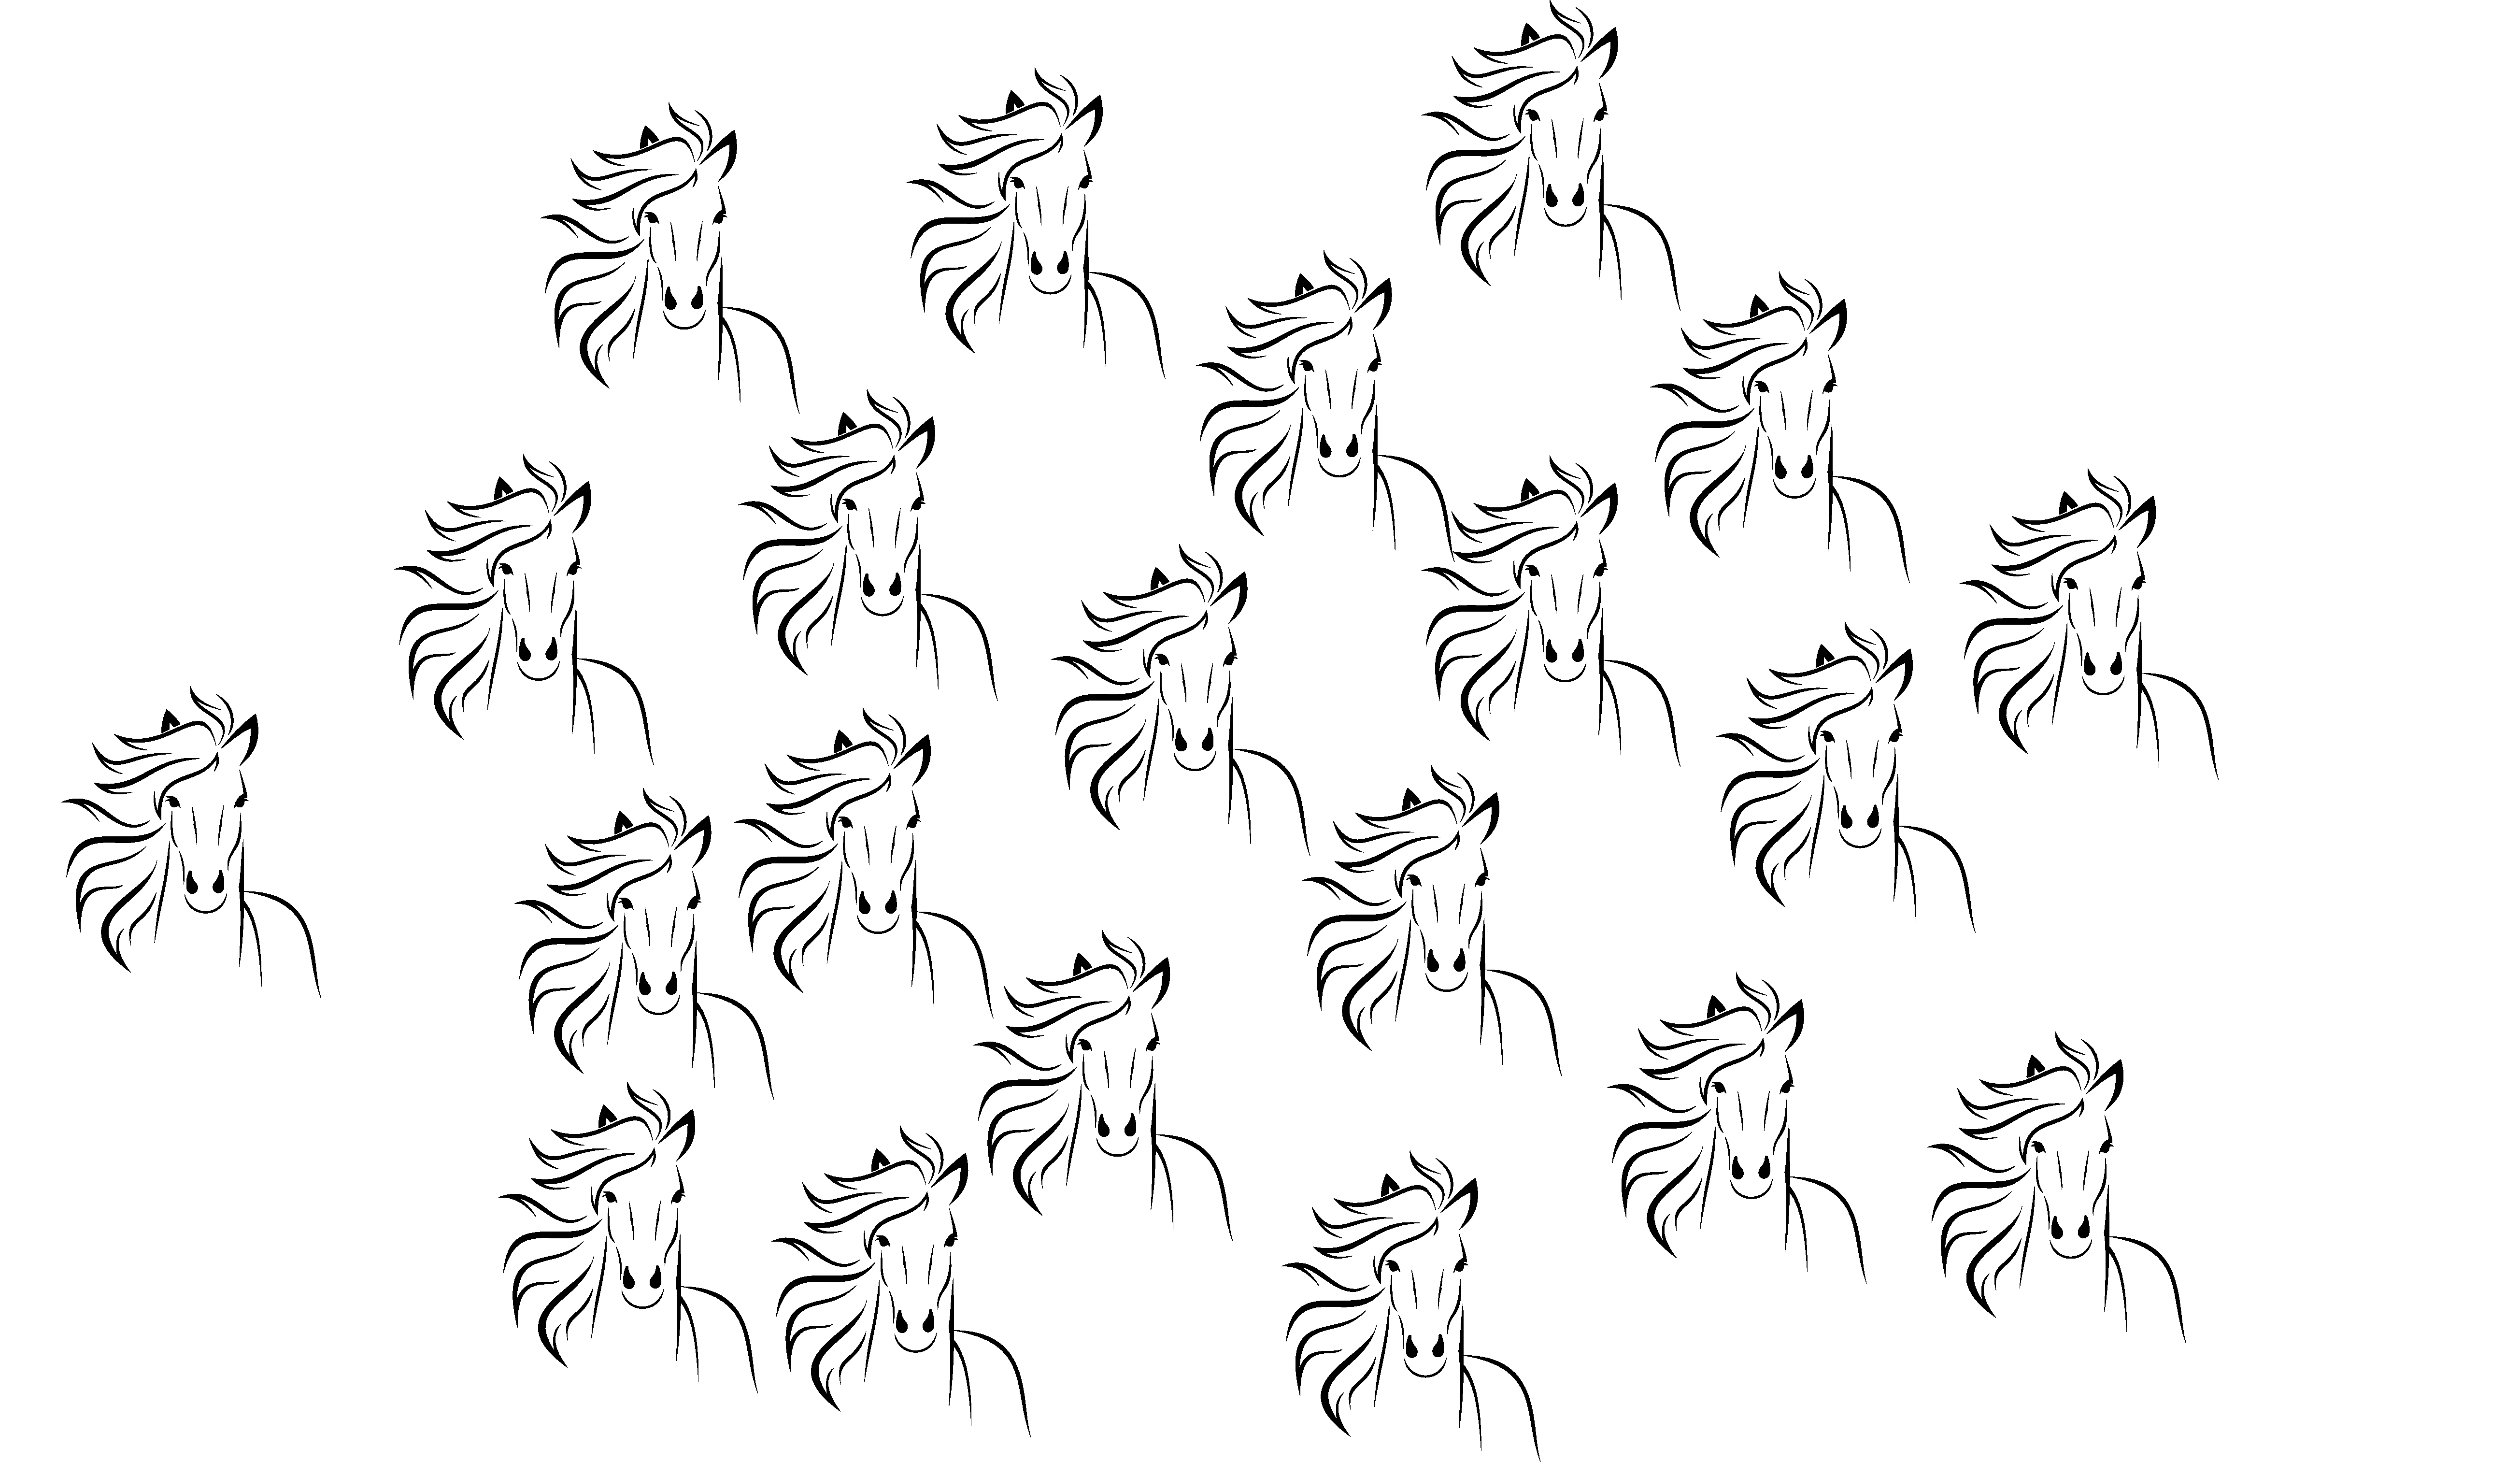
\includegraphics[height=2.5in]{pferd-weiss-remR}}%
 \only<7>{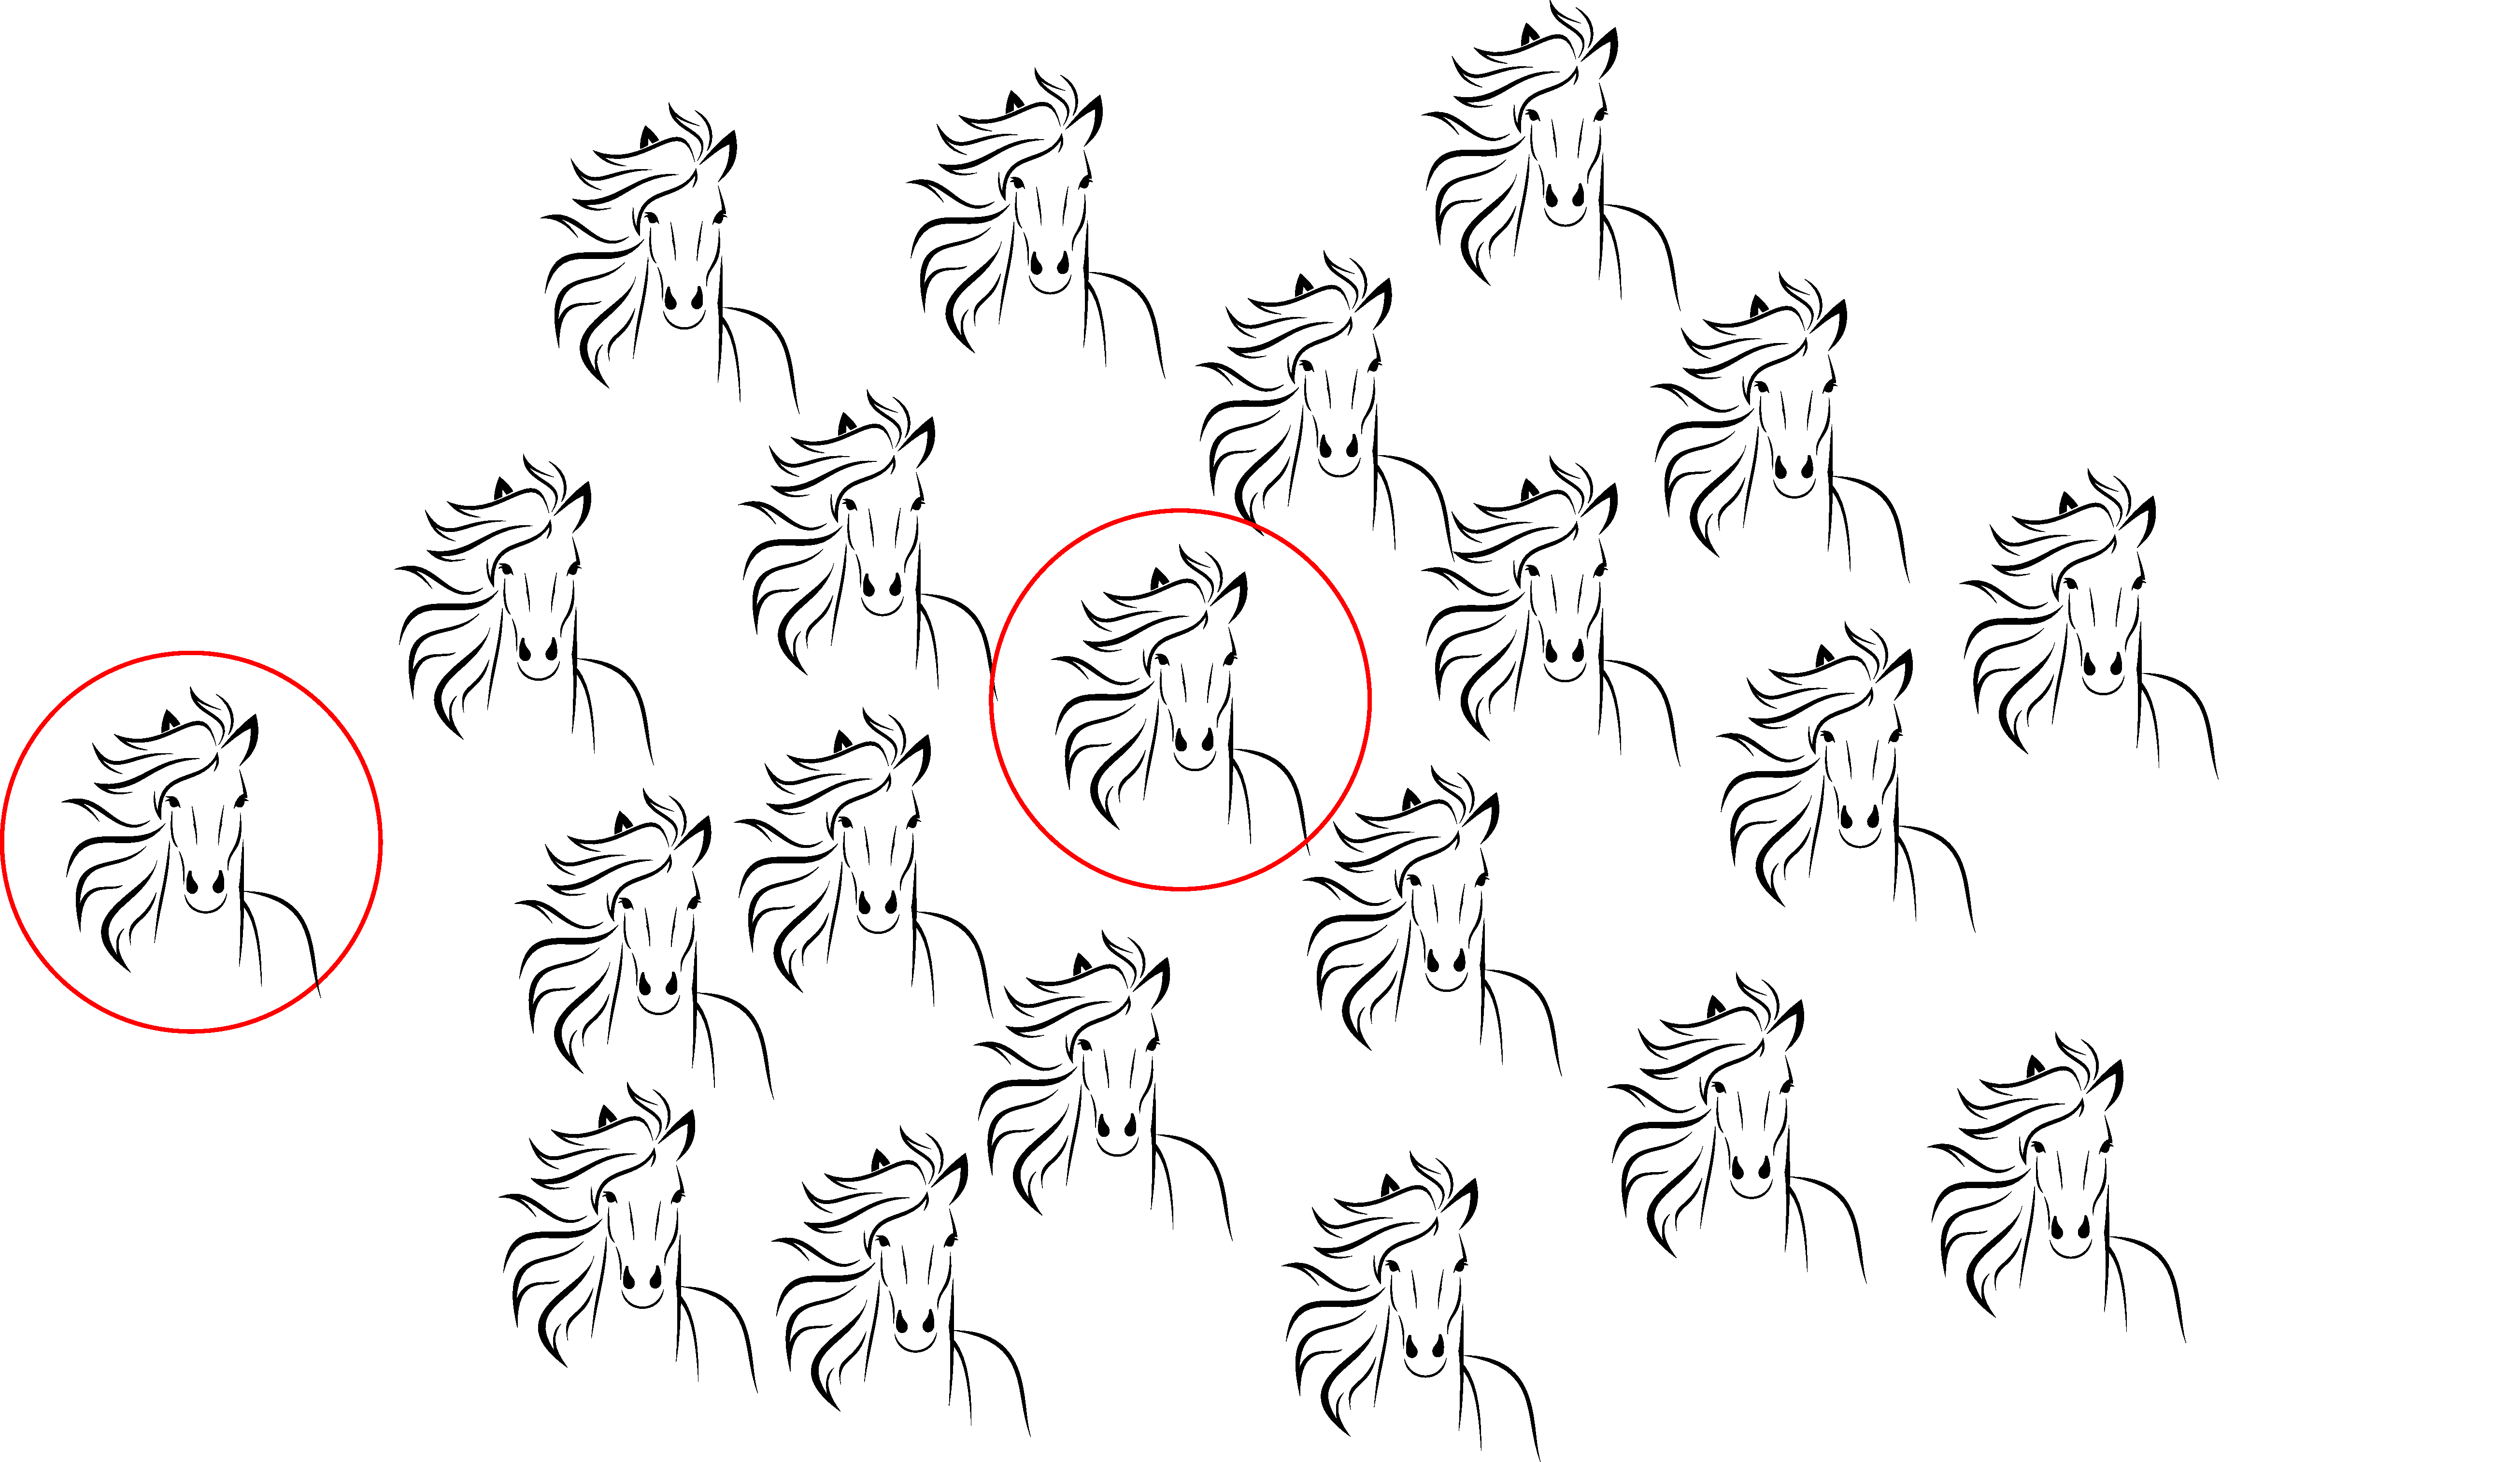
\includegraphics[height=2.5in]{pferd-weiss-L}}%
 \only<8>{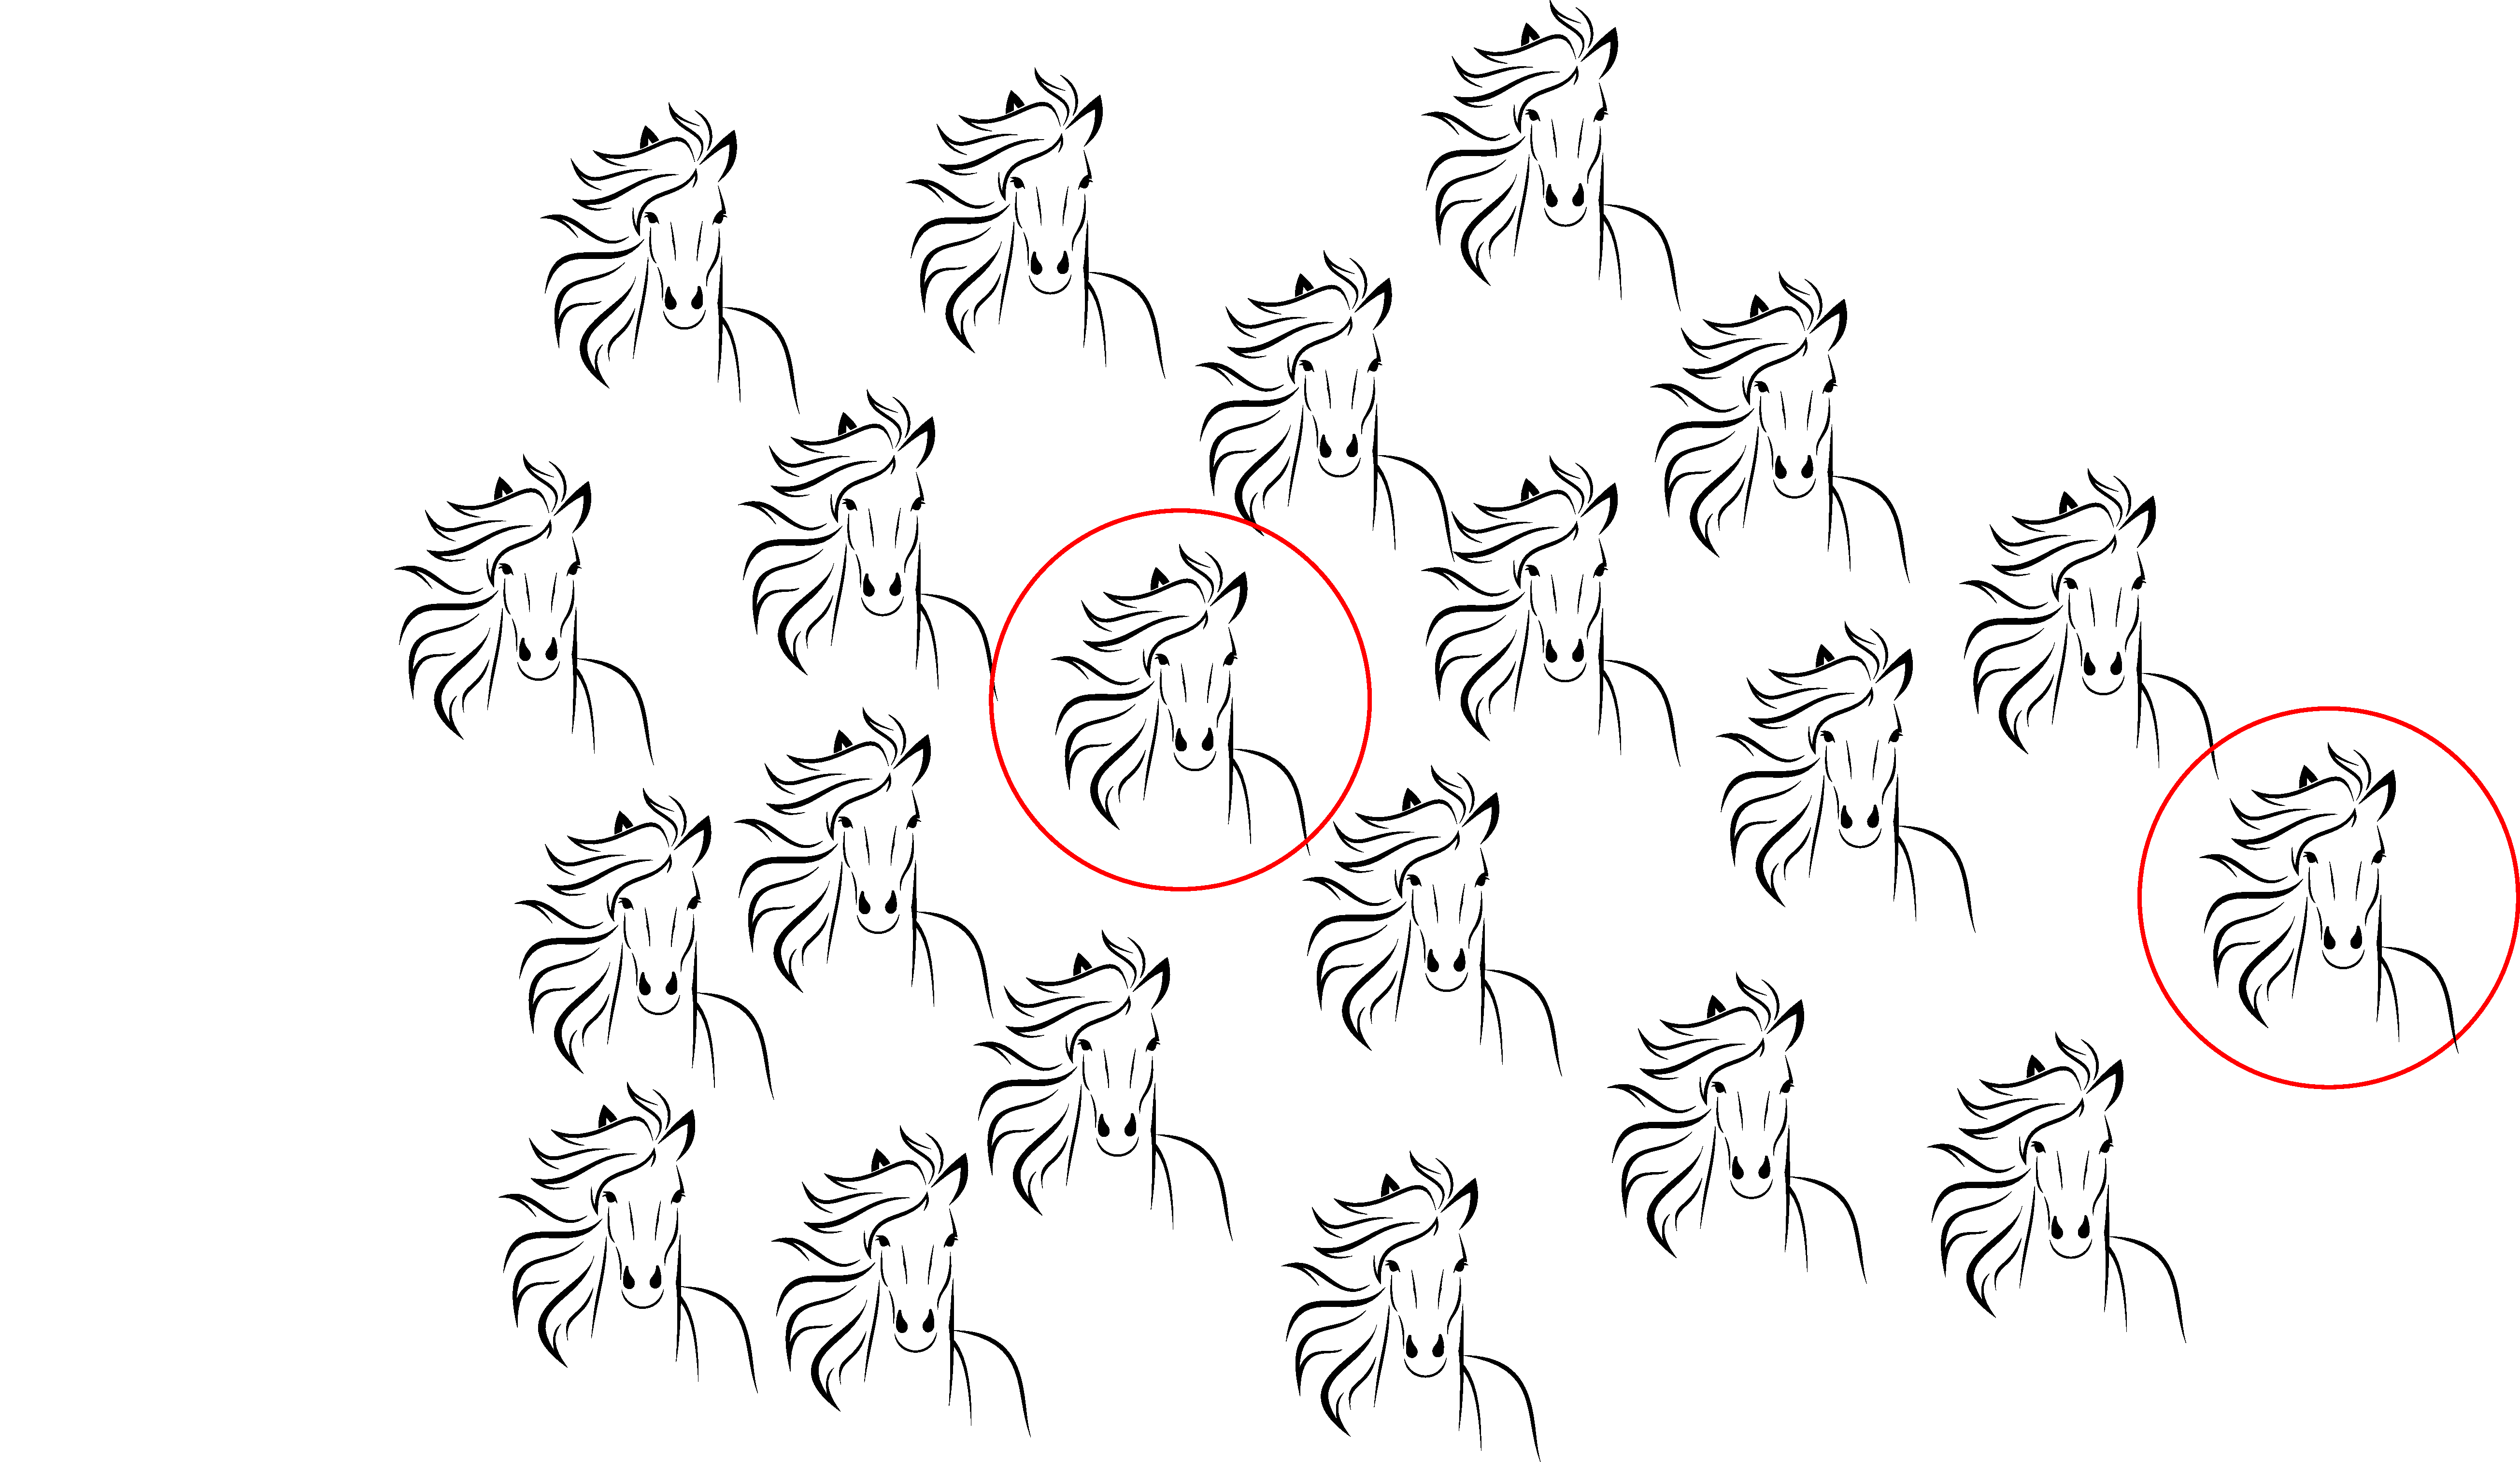
\includegraphics[height=2.5in]{pferd-weiss-R}}%
 \only<9->{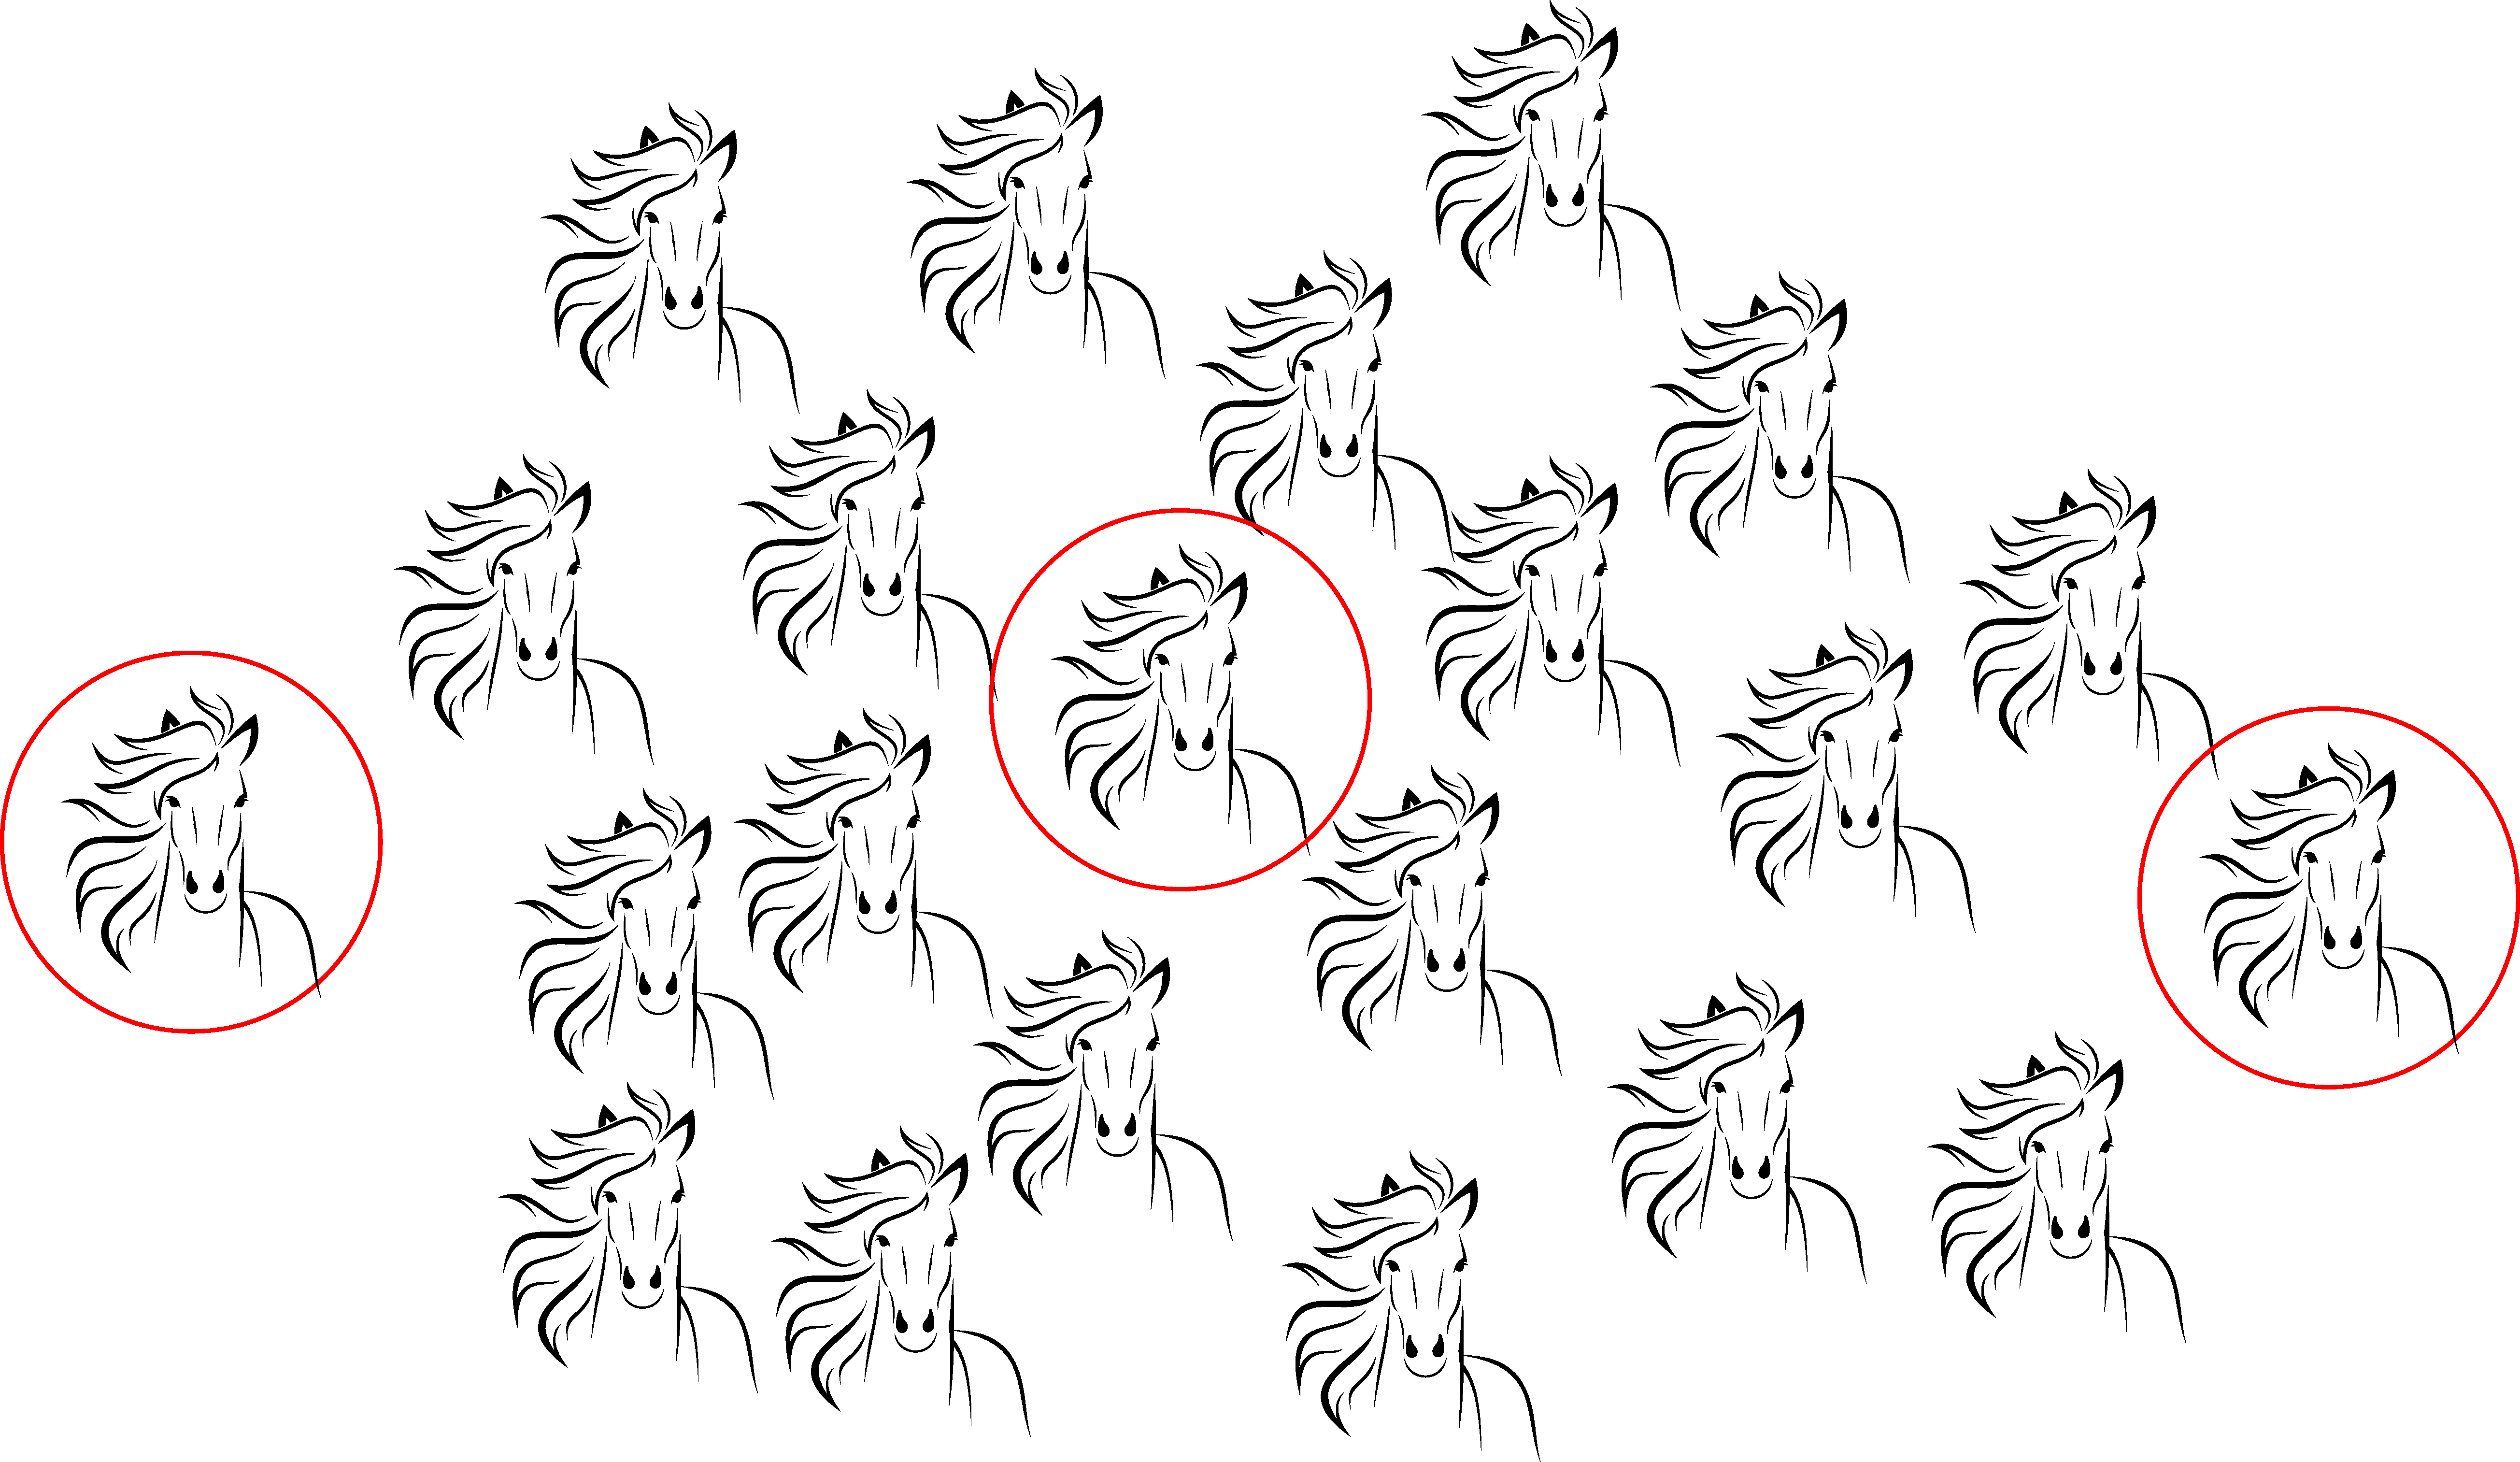
\includegraphics[height=2.5in]{pferd-weiss-all}}%
 \\
 \footnotesize{Pferd-weiss by marauder (openclipart)}
\end{block}

}

\againframe<3>{horseinduction}

\frame{

\begin{block}{Thank You!}
Email me: brittany@fasy.us
\end{block}

}

\frame{
\frametitle{Welcome to CSCI 432!}

\begin{block}{Horse Humor}
    Suppose we define a horse's tail to be a leg.\\
    How many legs does a horse have?"\pause
    \begin{itemize}
        \item The mathematician answers ``5";\pause
        \item the computer scientist ``1";\pause
        \item and the engineer says ``But you can't do that!"
    \end{itemize}
\end{block}

}

\end{document}
